\documentclass[dissertation.tex]{subfiles} 
\begin{document}

\chapter{Event Selection}
\label{chap:Event Selection}

In keeping with the phenomenology described in Sec.~\ref{sec:Phenomenology of General Gauge Mediation}, the candidate GGM events selected in this search consist of two high-$E_{T}$ photons and a significant momentum imbalance transverse to the beam, indicating the production of an escaping gravitino.  This momentum imbalance is usually referred to as \textit{missing transverse energy} and is denoted by the symbols \MET or $\mbox{ME}_{\mathrm{T}}$.  The GGM signature is shown in Figure~\ref{fig:GGM_diphoton_signal_Feynman_diagram}.

\begin{figure}
	\centering
	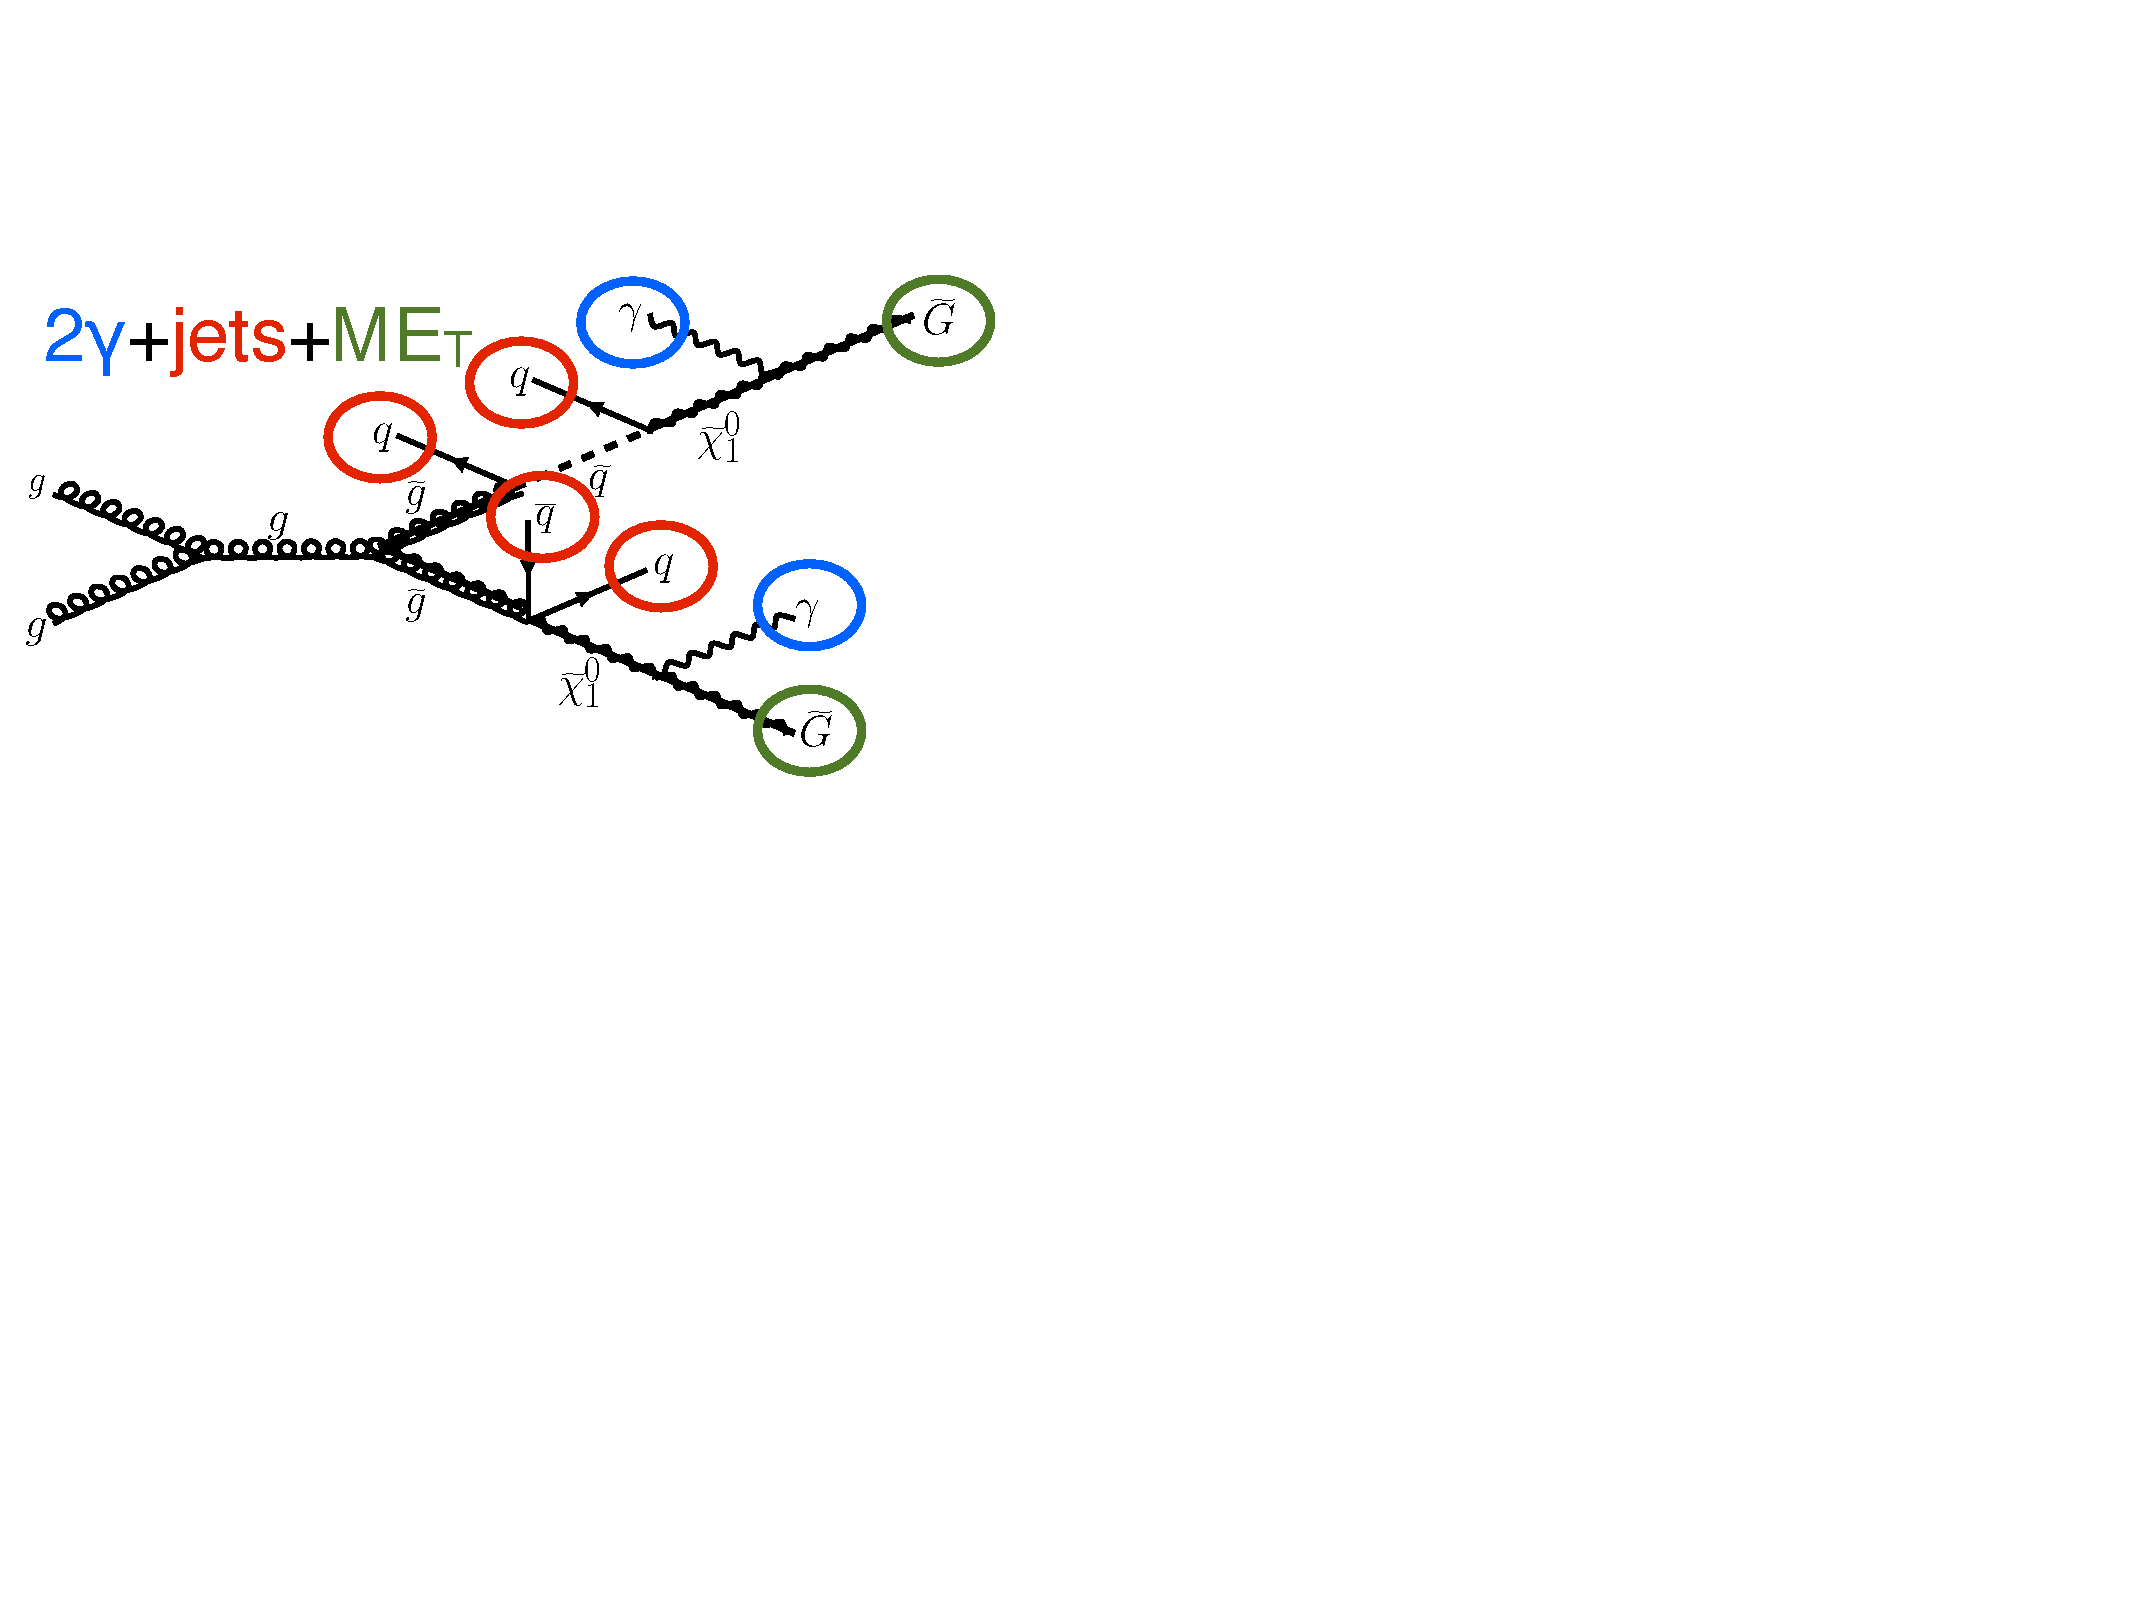
\includegraphics[scale=0.7]{2photons_jets_MET}
	\caption{Two gluinos each decay via $\NLSP\rightarrow\gamma\widetilde{G}$.}
	\label{fig:GGM_diphoton_signal_Feynman_diagram}
\end{figure}

However, in order to use real CMS data (as opposed to simulation) to derive predictions for the backgrounds to the search, \textit{control samples} that are not expected to contain any GGM signal events and are distinct from the \textit{candidate} two-photon sample must be collected from the LHC data.  These samples consist of different numerical combinations of photons, electrons, and jets, and are explained in more detail in Chapter~\ref{chap:Data Analysis}.  Since this search is performed in the high-\MET tail of the \MET distribution, where adequate detector simulation is very difficult, it is advantageous to use \textit{data-driven} background estimates, which capture the true detector response, over numbers derived from simulation.

In the following sections, the reconstruction of photons, electrons, jets, and \MET is explained.  Sec.~\ref{sec:Object Reconstruction} begins with an explanation of the high level reconstruction.  It is followed by Sec.~\ref{sec:HLT}, which describes the triggers used to collect the candidate and control samples.  Sec.~\ref{sec:Event Quality} describes event cleaning cuts that are applied to the candidate and control samples.  Finally, the chapter concludes with a measurement of the photon identification efficiency in Sec.~\ref{sec:Photon Identification Efficiency}.

\section{Object Reconstruction}
\label{sec:Object Reconstruction}

This section describes the \textit{offline} object reconstruction, i.e. the reconstruction of particle objects from events that have already been triggered and written to permanent storage, as opposed to the building of trigger objects explained in Secs.~\ref{sec:Level 1 and High Level Trigger Systems} and~\ref{sec:HLT}.

\subsection{Photons}
\label{sec:Photons}

\subsubsection{Uncalibrated EB/EE Hits}
\label{sec:Uncalibrated EB/EE Hits}

Photon reconstruction begins with the ADC count value for each of the 10 recorded time samples per ECAL crystal per trigger.  To construct an \textit{uncalibrated hit}, the gain (1, 6, or 12; see Sec.~\ref{sec:Electromagnetic Calorimeter}) of each sample is determined and the ADC count value scaled appropriately.  The pedestal is estimated from the average of the first three samples, which, for a properly timed in hit, should contain no signal.  This pedestal value is subtracted from the rest of the samples.  Finally, the amplitude of the pulse is reconstructed using a predetermined weight for each sample \cite{Bruneliere}.  The weights correspond to the pulse shape expected from the MGPA and shaping circuit response.  The time of the hit is also reconstructed using the ratios between neighboring time samples \cite{time_reco}.  A typical ECAL channel pulse shape is shown in Figure~\ref{fig:pulse}.

\begin{figure}
	\centering
	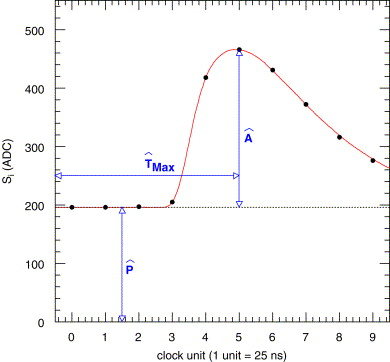
\includegraphics[scale=4.0]{pulse}
	\caption{Typical ECAL channel pulse shape.  $\widehat{P}$ is the pedestal value, $\widehat{A}$ is the pulse amplitude, and $\widehat{T}_{\mathrm{max}}$ is the hit time.  The red line is the assumed pulse shape from which the weights are derived.  Reprinted from ref. \cite{Bruneliere}.}
	\label{fig:pulse}
\end{figure}

\subsubsection{Calibrated EB/EE Hits}
\label{sec:Calibrated EB/EE Hits}

In the next phase of the photon reconstruction, calibrations are applied to the uncalibrated hits to form \textit{calibrated hits} with energy measured in GeV.  Channels are excluded from seeding calibrated hits if

\begin{itemize}
\item they are excessively noisy,
\item they are stuck in fixed gain (i.e. the MGPA gain does not change properly to avoid saturation),
\item they are totally dead,
\item they have one or more neighboring dead channels, or
\item they do not have good trigger primitives (i.e. trigger primitive is missing, saturated, or \textit{spike-like}; cf. Secs.~\ref{sec:Electromagnetic Calorimeter} and~\ref{sec:Level 1 and High Level Trigger Systems}).
\end{itemize}

\marginpar{\textcolor{blue}{Added this paragraph and the next about spikes}}\textit{ECAL spikes} are hits in which low energy protons and heavy ions from jets ionize in the sensitive volume of the EB APD (Sec.~\ref{sec:Electromagnetic Calorimeter}), causing the APD to register a fake large-amplitude hit.  Because they are not the result of a real electromagnetic shower, spikes tend to be isolated.  They may also appear to arrive early or late with respect to the nominal bunch crossing.  Most spikes are reconstructed with a hit time $\sim$10 ns earlier than real EM hits because unlike real hits, whose pulse shapes include the time constant associated with crystal scintillation, the reconstructed spikes only involve the rise time of the electronics.  There also is a long tail of late arriving spikes due to slow neutrons from jets \cite{EGM_10_002}.

Because of their particular timing and topological characteristics, cuts have been developed to effectively identify and reject spike-like hits.  This analysis utilizes both the ``Swiss cross" cut 1 - $E_{4}/E_{1} >$ 0.95, where $E_{1}$ is the energy of the spike candidate crystal and $E_{4}$ is the sum of the energies in the four crystals whose edges are next to the four edges of the spike candidate crystal, and a timing cut $t \geq$ 3 ns, to flag spikes.  More information about these cuts can be found in ref. \cite{EGM_10_002}.  A simpler algorithm using the fine grain veto bit of the ECAL L1 TPG (Sec.~\ref{sec:Level 1 and High Level Trigger Systems}) is used to reject spikes at the trigger level.

In addition to the trigger primitives, no uncalibrated hits that are spike-like are eligible for calibration.  The calibrations applied are corrections to account for crystal transparency and VPT photocathode loss (leading to signal loss), measured continuously by the laser/LED system; energy intercalibrations (relative energy calibration between crystals); absolute scale calibrations between ADC counts and GeV;\footnote{The ADC-GeV scale factors (one for EB and one for EE) are defined such that the sum of fully calibrated and scaled hits in a particular 5 $\times$ 5 cluster of crystals (plus the associated energy deposited in ES) is 50 GeV for a 50 GeV incident unconverted photon \cite{calibration_IN}.} and time intercalibrations (relative time calibration between crystals).

The ECAL crystals were pre-calibrated before installation in CMS using laboratory light yield and photodetector gain measurements \cite{EB_performance_2006}.  In addition, some EB and EE crystals were intercalibrated using test beams \cite{EB_startup_intercalibration}, and all EB crystals were intercalibrated with cosmic ray muons \cite{CRAFT_calibration}.  EE precalibrations were validated with LHC \textit{splash events} in 2009 \cite{CRAFT_calibration, CRAFT_ECAL_performance}, in which the beam was dumped onto a collimator approximately 150 meters upstream of CMS, causing a spray of muons to enter CMS at one endcap and exit at the other.  Splash events were also used to derive time intercalibration constants.  Before colliding beam operations commenced, the intercalibration precision was estimated to be 0.5\%-2.2\% in EB and 1\%-5\% in EE \cite{CALOR_ECAL_calibration}.

Three calibration methods were employed once colliding beam operations began:

\begin{itemize}
\item $\phi$ symmetry relative calibration between crystals, exploiting the azimuthal symmetry of CMS
\item $\pi^{0}$ and $\eta$ relative calibration between crystals, using the diphoton decays of these particles
\item $E/p$ absolute calibration, comparing the momentum measured in the tracker $p$ to the energy measured in the ECAL $E$ of a sample of electrons from $Z$ decay
\end{itemize}
%
By September 2011, the intercalibration precision in EB was measured to be between 0.3\% and 1.1\% using the $\pi^{0}/\eta$ method \cite{Yang}.  Figure~\ref{fig:intercalibration} shows the improvement in $Z$ reconstruction from pre-LHC calibration constants to the latest $\pi^{0}/\eta$-derived constants.

\begin{figure}
	\centering
	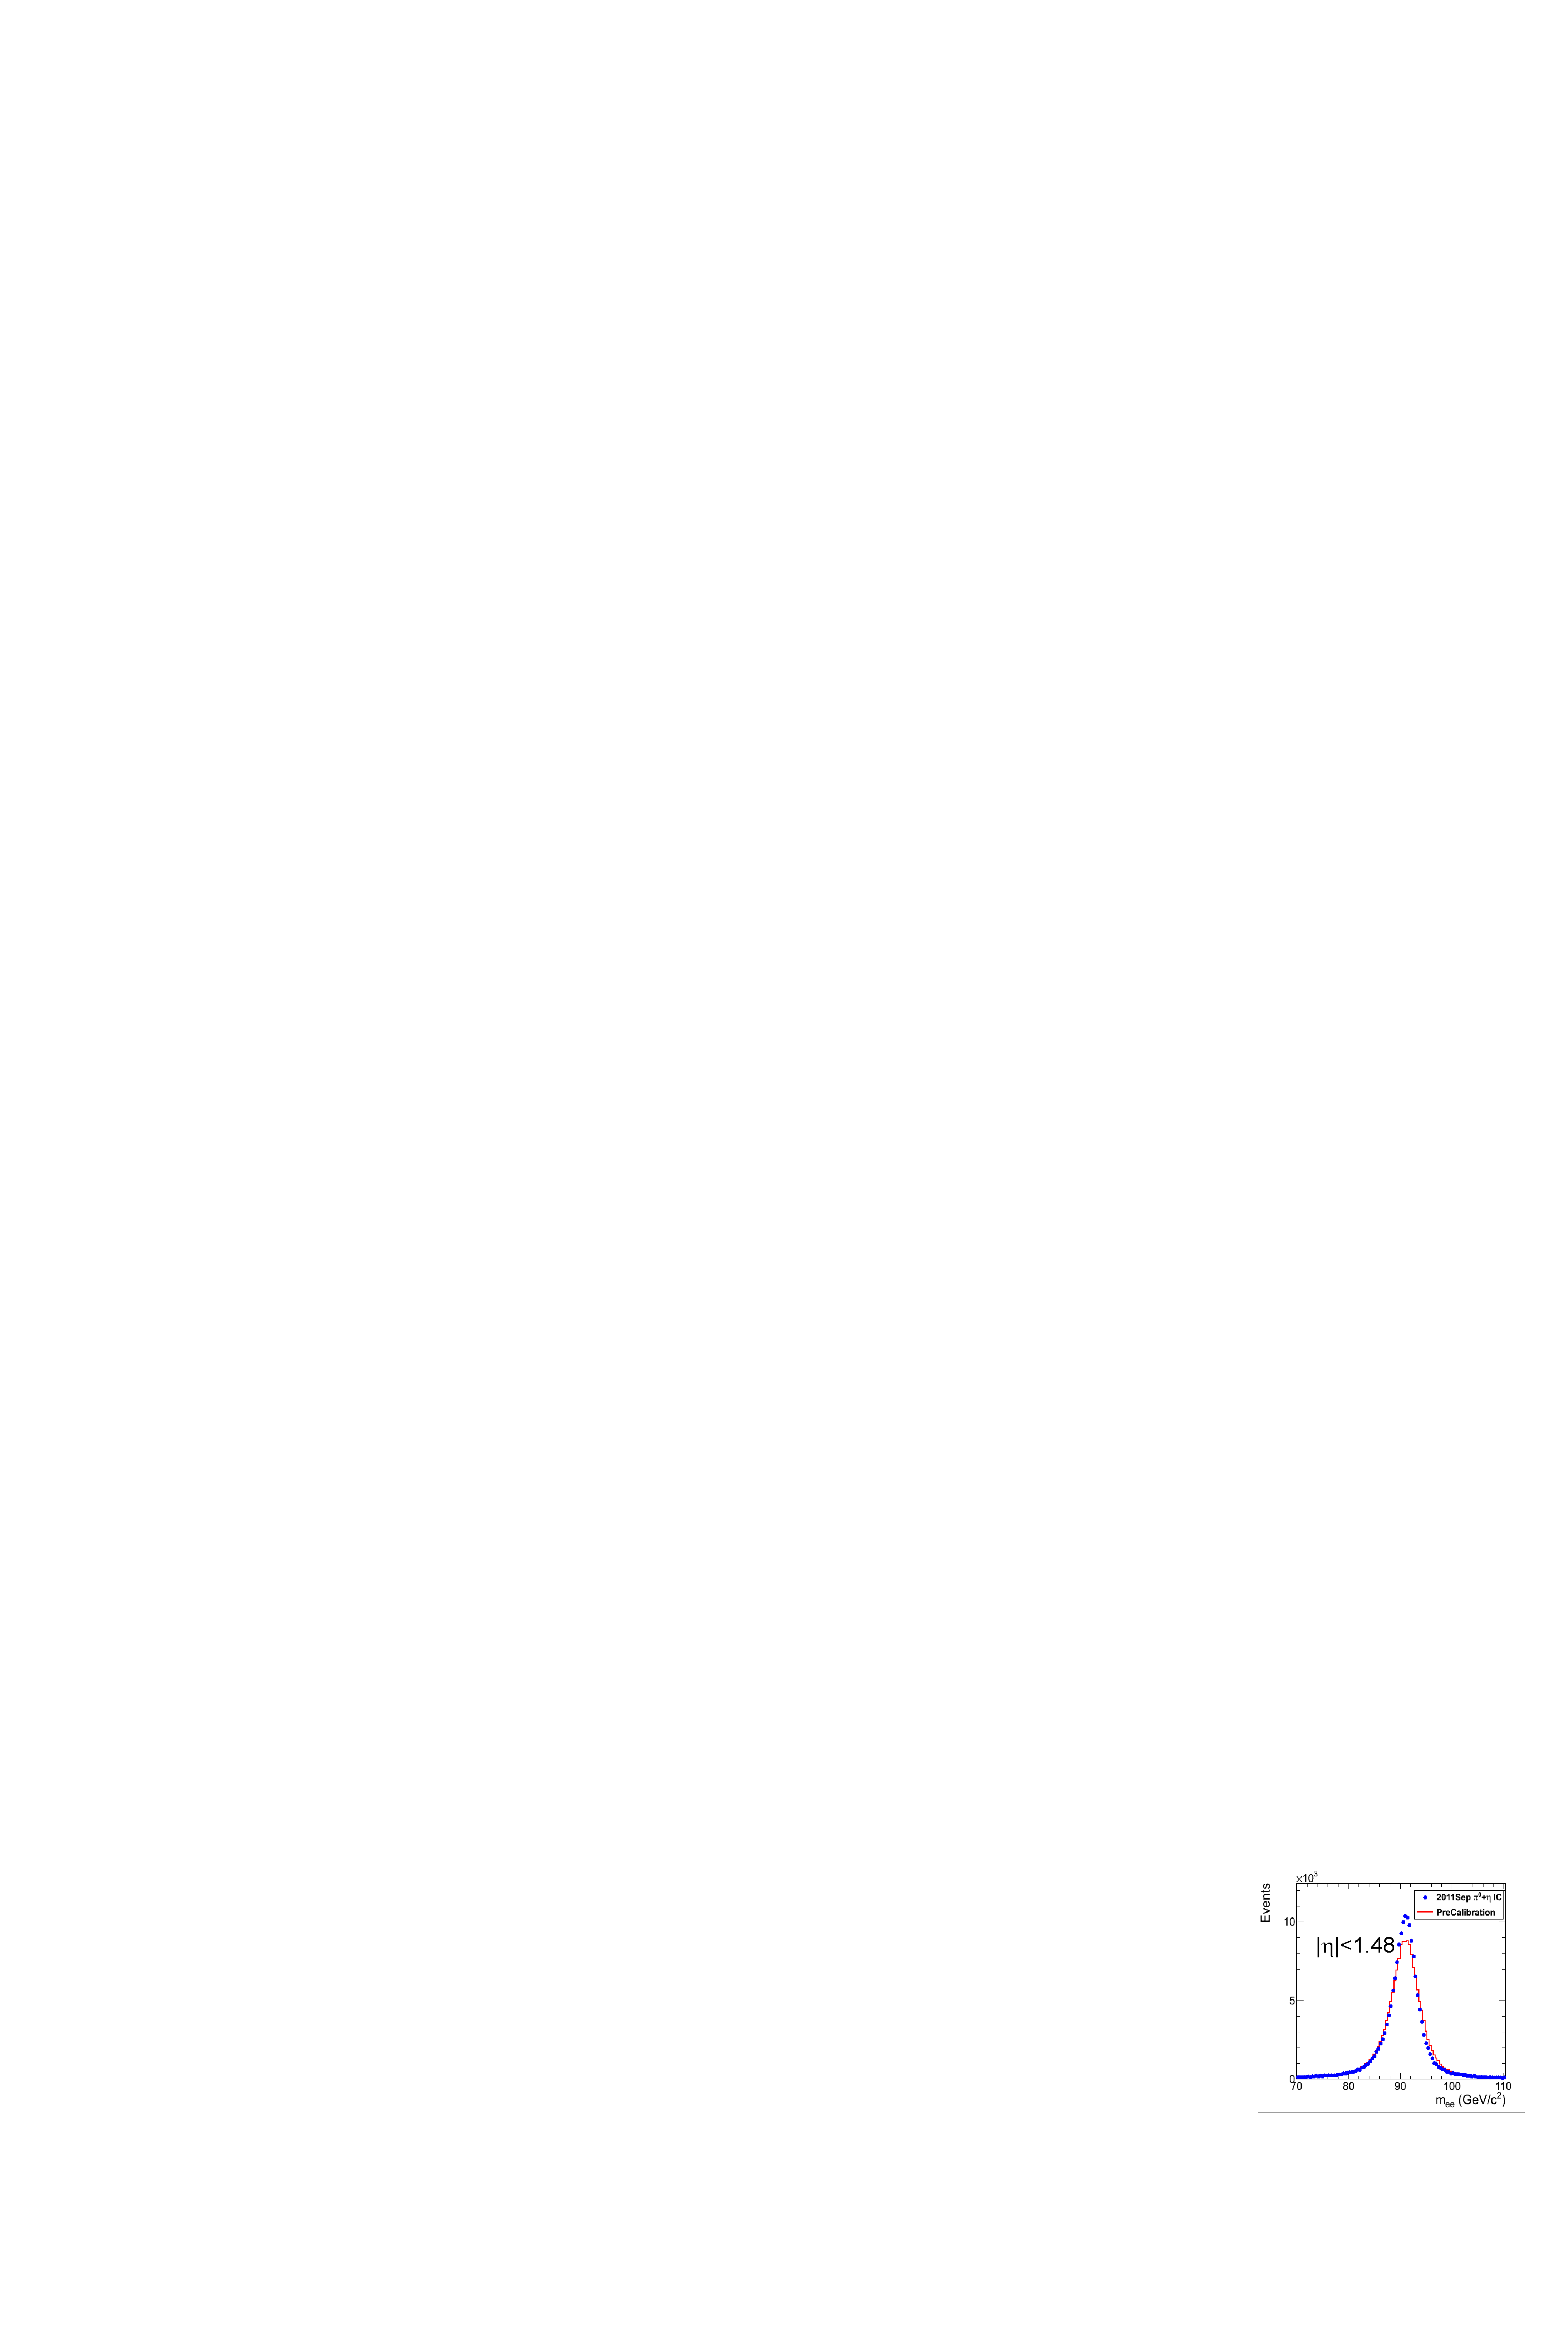
\includegraphics[scale=1.0]{intercalibration}
	\caption{$Z$ peak reconstructed using pre-LHC calibration constants (red) or September 2011 $\pi^{0}/\eta$-derived intercalibration constants (blue).  Reprinted from ref. \cite{Yang}.}
	\label{fig:intercalibration}
\end{figure}

\subsubsection{Calibrated ES Hits}
\label{sec:Calibrated ES Hits}

\marginpar{\textcolor{blue}{Added parenthetical remark}}ES calibrated hits are formed from the three samples read out per sensor.  Just as in the case of EB/EE crystals, ES uncalibrated hits are gain-adjusted, pedestal-subtracted, and reconstructed using weights.  To make a calibrated ES hit, intercalibration constants, angle correction constants (for the non-uniformity of sensor angle with respect to the vertical across ES), and a MIP-GeV absolute scale factor are applied.

\subsubsection{Clustering}
\label{sec:Clustering}

After calibrated ECAL hits are formed, they must be clustered into shapes that represent the energy deposit from a single particle.  \textit{Basic clusters} are formed around seed hits, defined as a hit that

\begin{itemize}
\item has calibrated $E_{T} >$ 1(0.18) GeV in EB(EE),
\item does not originate from a dead channel or one with faulty hardware,
\item is not poorly calibrated,
\item was reconstructed with the standard algorithm (i.e. not a special recovery algorithm for channels with subpar data integrity),
\item is not saturated,
\item is not spike-like, and
\item is in time (EB).
\end{itemize}
%
EB basic clusters are formed around the seeds via the \textit{hybrid} algorithm, while EE basic clusters are formed with the \verb+multi5x5+ algorithm \cite{ECAL_SC_note}.  In addition to handling non-radiating electrons and unconverted photons, both algorithms are designed to also recover all of the energy associated with electron bremsstrahlung deposits and photon conversions.  The geometry of the CMS magnetic field means that bremsstrahlung and conversions will tend to spread the shower out in $\phi$, not $\eta$.  Both algorithms work by forming basic clusters around seeds, then combining the basic clusters into \textit{superclusters} (SC) by searching in a window extended in the $\phi$ direction for all basic clusters consistent with bremsstrahlung radiation from the primary electron, or with a photon conversion.  Figure~\ref{fig:hybrid} illustrates the hybrid algorithm in EB.  In EE, the energy deposited in ES must also be added into the total clustered energy sum.

\begin{figure}
	\centering
	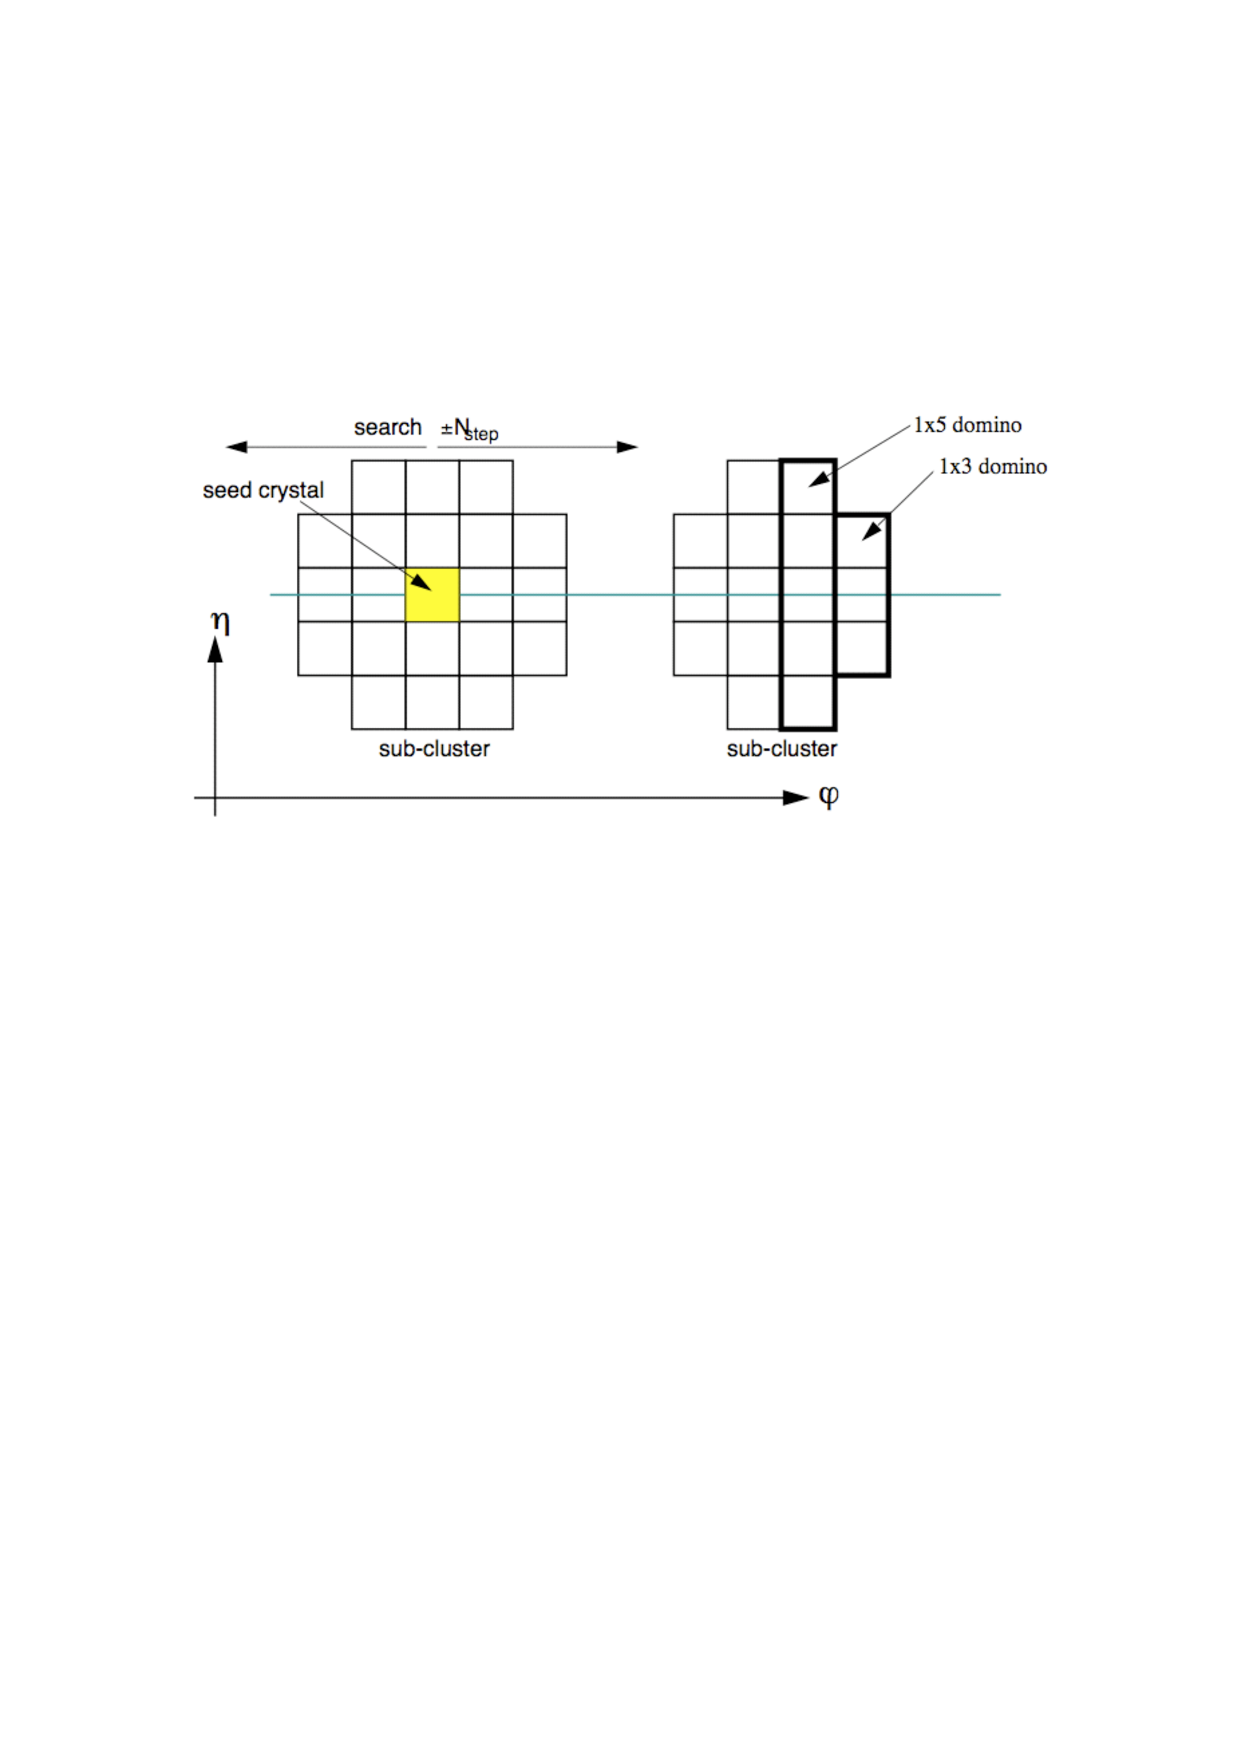
\includegraphics[scale=1.0]{hybrid}
	\caption{Hybrid algorithm in EB.  The shower extent is constant in $\eta$ (five crystals), but spreads out in $\phi$ as the two sub-clusters (or basic clusters) are grouped into the same supercluster.  The maximum extent in $\phi$ is 17 crystals.  Reprinted from ref. \cite{ECAL_SC_note}.}
	\label{fig:hybrid}
\end{figure}

Figure~\ref{fig:Z_mass_vs_corrections} shows the effect of superclustering on $Z\rightarrow ee$ reconstruction.

\begin{figure}
	\centering
	\subfloat[EB.]{\label{fig:Z_mass_vs_corrections_EB}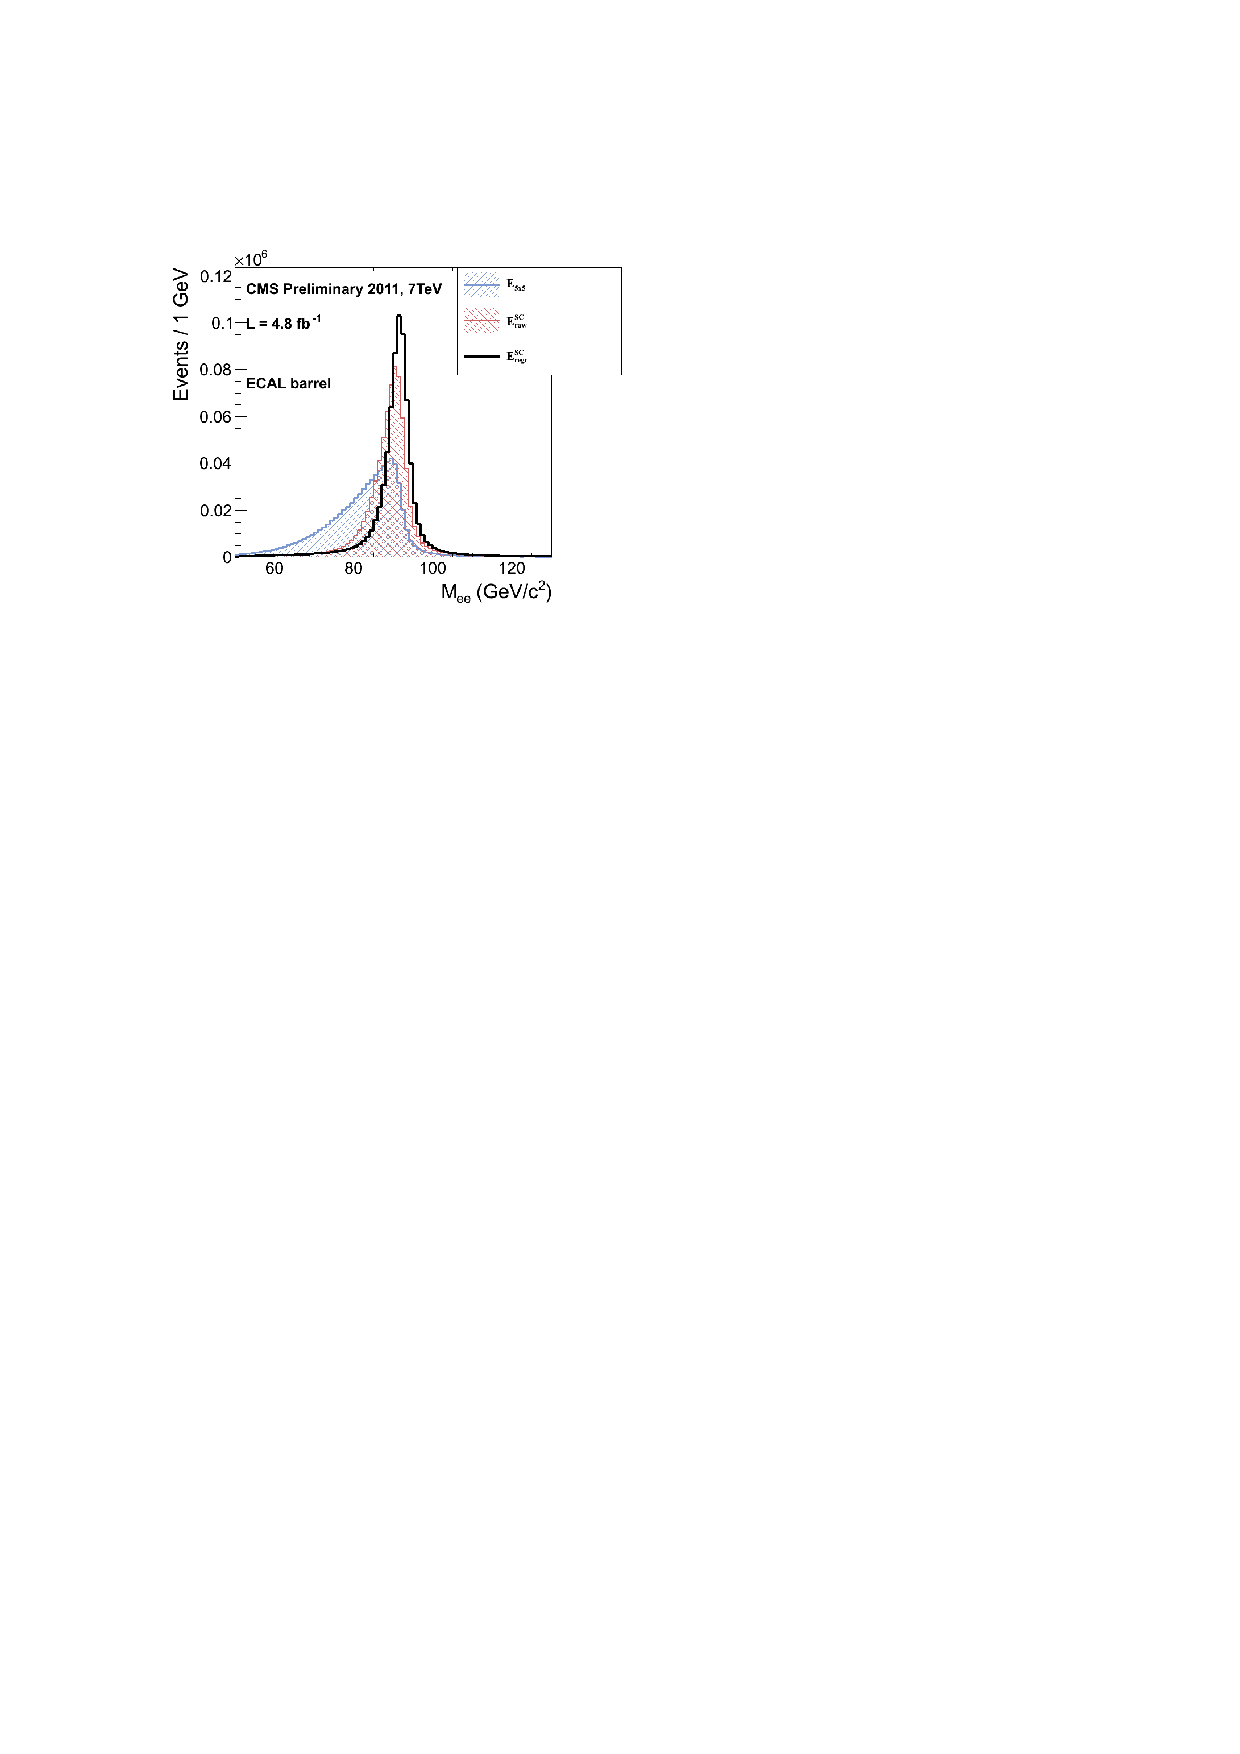
\includegraphics[scale=1.2]{Z_mass_vs_corrections_EB}}
	\\
	\subfloat[EE.]{\label{fig:Z_mass_vs_corrections_EE}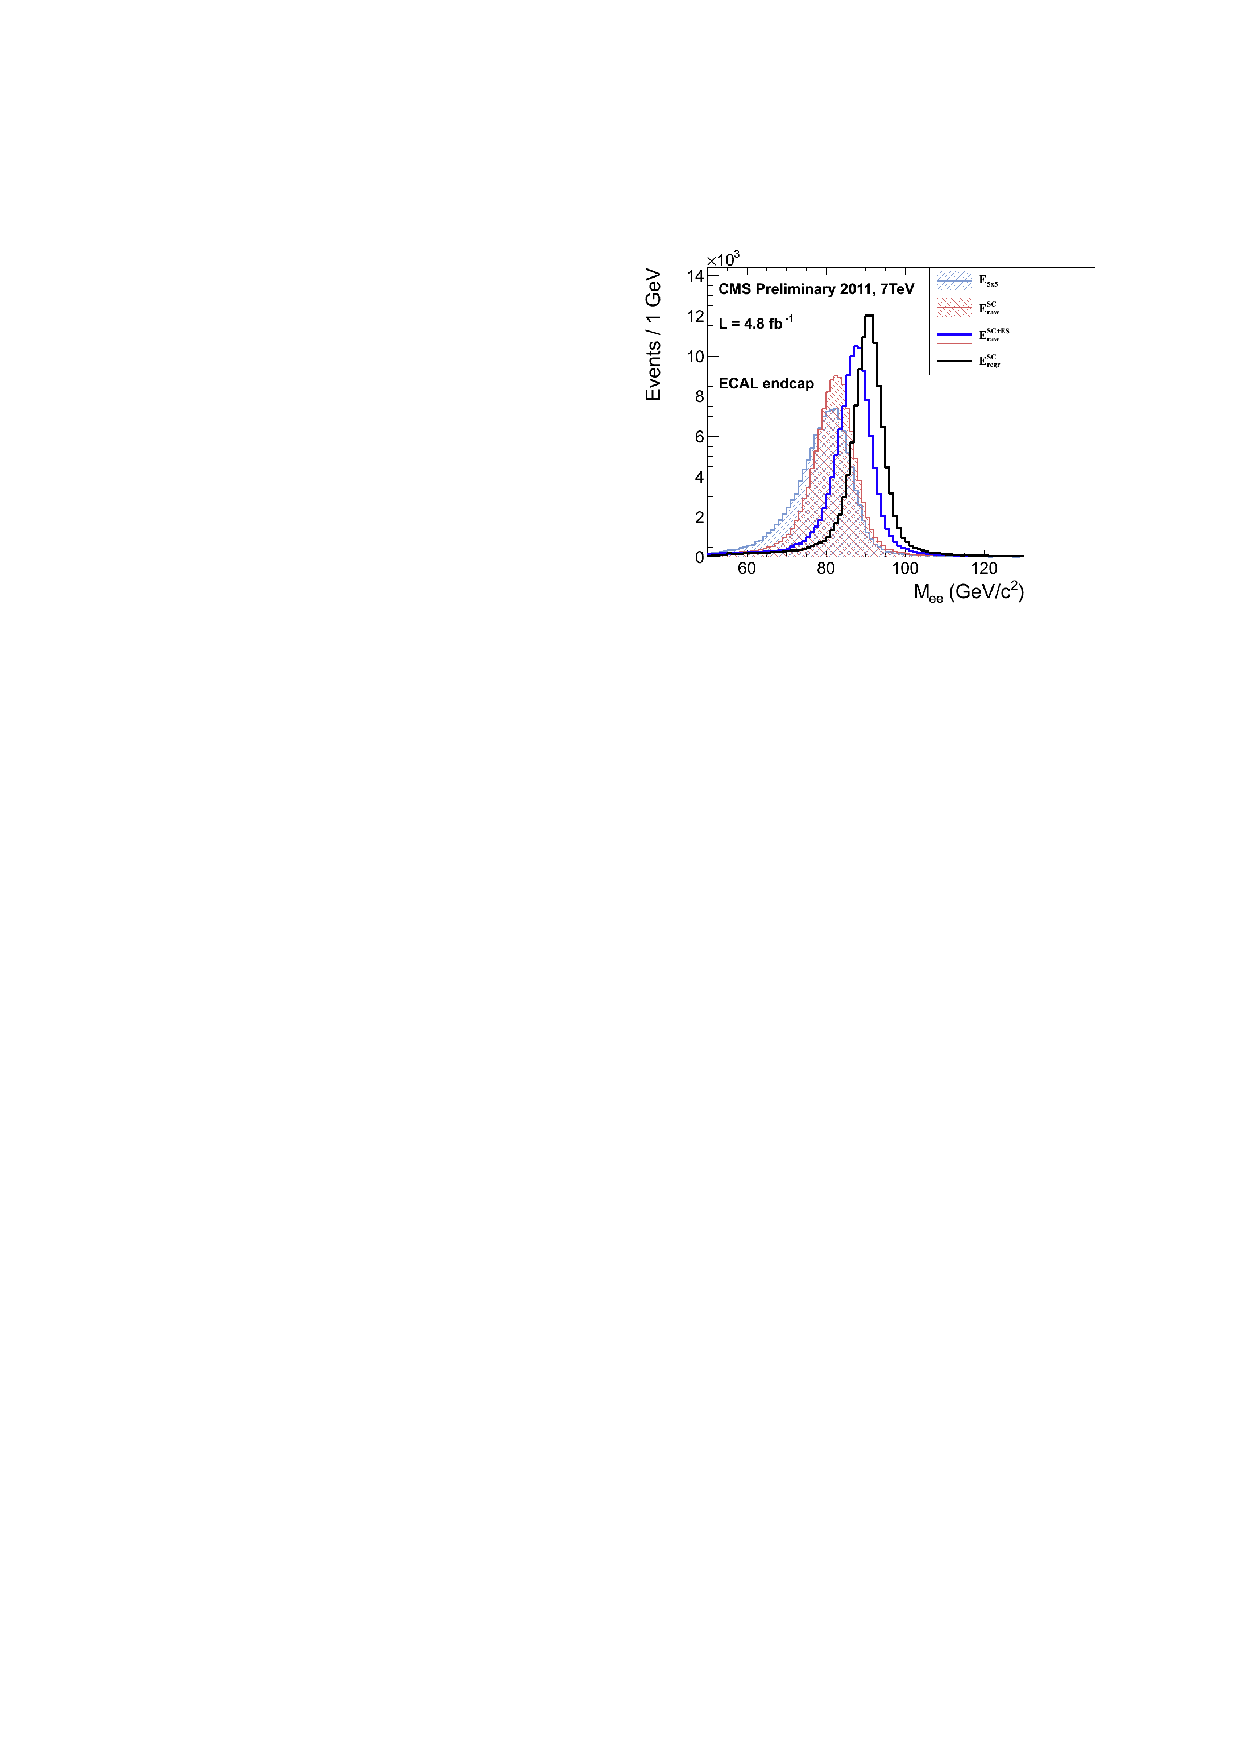
\includegraphics[scale=1.2]{Z_mass_vs_corrections_EE}}
	\caption{$Z$ peak reconstructed in the dielectron channel for different kinds of clustering.  The constituent hits were calibrated with the best available intercalibrations and laser calibrations as of December 2011.  The light blue histogram shows the reconstruction using a 5 $\times$ 5 energy sum, the red histogram shows the reconstruction using the SC energy for crystals only (the dark blue histogram in the EE plot adds in the energy from ES), and the black histogram shows the reconstruction after the SCs are corrected using a multivariate method \cite{Higgs_AN}.  Reprinted from Fig. 30 of ref. \cite{Higgs_AN}.}
	\label{fig:Z_mass_vs_corrections}
\end{figure}

\subsubsection{Supercluster Corrections}
\label{sec:Supercluster Corrections}

The total clustered ECAL energy is defined as

\begin{eqnarray}
E &=& F \times \sum_{i=1}^{n_{\mathrm{crystal}}} G \times c_{i} \times A_{i}
\end{eqnarray}
%
where $G$ is the ADC-GeV or MIP-GeV scale factor, $c_{i}$ are the intercalibration constants, $A_{i}$ is the uncalibrated hit amplitude in ADC counts, and $F$ is a SC correction factor.  $G$ and $c_{i}$ were explained in Sec.~\ref{sec:Calibrated EB/EE Hits}.  $F$ is a product of three factors for hybrid SCs (two for \verb+multi5x5+ SCs in EE, items 2 and 3 below) \cite{ECAL_SC_note}:

\begin{enumerate}
  \item $C_{\mathrm{EB}}(\eta)$, which compensates for lateral energy leakage due to the crystal off-pointing in EB only.  These corrections are taken from MC simulation \cite{ECAL_SC_note} and were confirmed in test beams \cite{EB_startup_intercalibration}.
  \item $f(\mbox{brem})$, which corrects for biases in the clustering algorithms for showers characterized by differing amounts of bremsstrahlung.  These corrections are taken from MC simulation \cite{ECAL_SC_note}.
  \item Residual correction $f(E_{T}, \eta)$, due to the variation in $\eta$ of detector material traversed by a primary electron or photon, and to any residual $E_{T}$ dependence of the reconstruction.  These corrections are determined from MC and validated on $Z\rightarrow ee$ data samples \cite{ECALEnergyScaleCorrections_Twiki}.\marginpar{\textcolor{blue}{Changed}}
\end{enumerate}

As a benchmark of ECAL calibration performance, the extra energy smearing in MC needed to achieve data/MC agreement in the $Z$ width was between $\sim$0.9\% (in the central part of EB for electrons with little bremsstrahlung) and $\sim$3.3\% (in the outer part of EE for heavily radiating electrons) \cite{Higgs_note}.

\subsubsection{From Supercluster to Photon}
\label{sec:From Supercluster to Photon}

The CMS photon object is any SC with $E_{T} > 10$ GeV and $H/E < 0.5$, unless the SC $E_{T} > 100$ GeV, in which case the $H/E$ requirement is dropped.  $H/E$ is defined as the ratio of energy in the HCAL in a 0.15 cone around the SC centroid, directly behind the SC, to the SC energy.  SCs with $R9 > 0.94(0.95)$ in EB(EE), where $R9$ is defined as the ratio of the energy in the central 3$\times$3 cluster of crystals divided by the SC energy $E_{3\times 3}/E_{\mathrm{SC}}$, are the best calibrated and most accurate type of electromagnetic shower.  Therefore, for these objects, the photon energy is defined as the energy sum of the fully calibrated hits in the central 5 $\times$ 5 cluster around the seed (with $C_{\mathrm{EB}}(\eta)$ applied for EB photons).  For all other SCs, the photon energy is equal to the fully corrected SC energy (cf. Sec.~\ref{sec:Supercluster Corrections}).

\marginpar{\textcolor{blue}{Reorganized next 3 paragraphs; edited Table~\ref{tab:g_f_criteria} caption}}In this search, candidate photons and \textit{fake photons} ($\mathit{f}$, ``fakes") are further selected according to the criteria listed in Table~\ref{tab:g_f_criteria}.  Fakes are used in the determination of the QCD background, as explained in Chapter~\ref{chap:Data Analysis}.

\begin{table}[hcbp]
\caption{Selection criteria for photons and fakes.  ``Pixel seed," $I_{\mathrm{comb}}$, and $\sigma_{i\eta i\eta}$ are defined in the text.}
\centering
\begin{tabular}{|c|c|c|}
\hline
Variable & Cut ($\gamma$) & Cut ($\mathit{f}$) \\
\hline
\hline
SC $|\eta|$ & $< 1.4442$ & $<1.4442$ \\
\hline
$H/E$ & $<0.05$ & $<0.05$ \\
\hline
$R9$ & $< 1$ & $< 1$ \\
\hline
Has pixel seed & No & No \\
\hline
$I_{\mathrm{comb}}$, $\sigma_{i\eta i\eta}$ & $< 6$ GeV AND $< 0.011$ & ($\geq 6$ AND $< 20$ GeV) OR $\geq 0.011$ \\
\hline
\end{tabular}
\label{tab:g_f_criteria}
\end{table}

\marginpar{\textcolor{blue}{Updated effective area}}$I_{\mathrm{comb}}$ is defined as

\begin{eqnarray}
I_{\mathrm{comb}} &=& I_{\mathrm{ECAL}} - 0.093\rho + I_{\mathrm{HCAL}} - 0.0281\rho + I_{\mathrm{track}}
\end{eqnarray}
%
where $I_{\mathrm{ECAL}}$, $I_{\mathrm{HCAL}}$, and $I_{\mathrm{track}}$ are $E_{T}$ sums in the annular regions defined in Figure~\ref{fig:isolation_cones} and $\rho$ is the average pileup energy density in the calorimeters (per unit $\eta\cdot\phi$, or unit calorimeter surface area) as measured with the Fastjet algorithm \cite{Fastjet_conf_proceedings, Fastjet_manual}.  $\rho$ is constant over the $\eta$ range of the calorimeter.  Note that the ECAL and track isolation veto strips at constant $\eta$ ensure that the isolation cuts are similarly efficient for converted photons, radiating electrons, and unconverted photons.

\begin{figure}
	\centering
	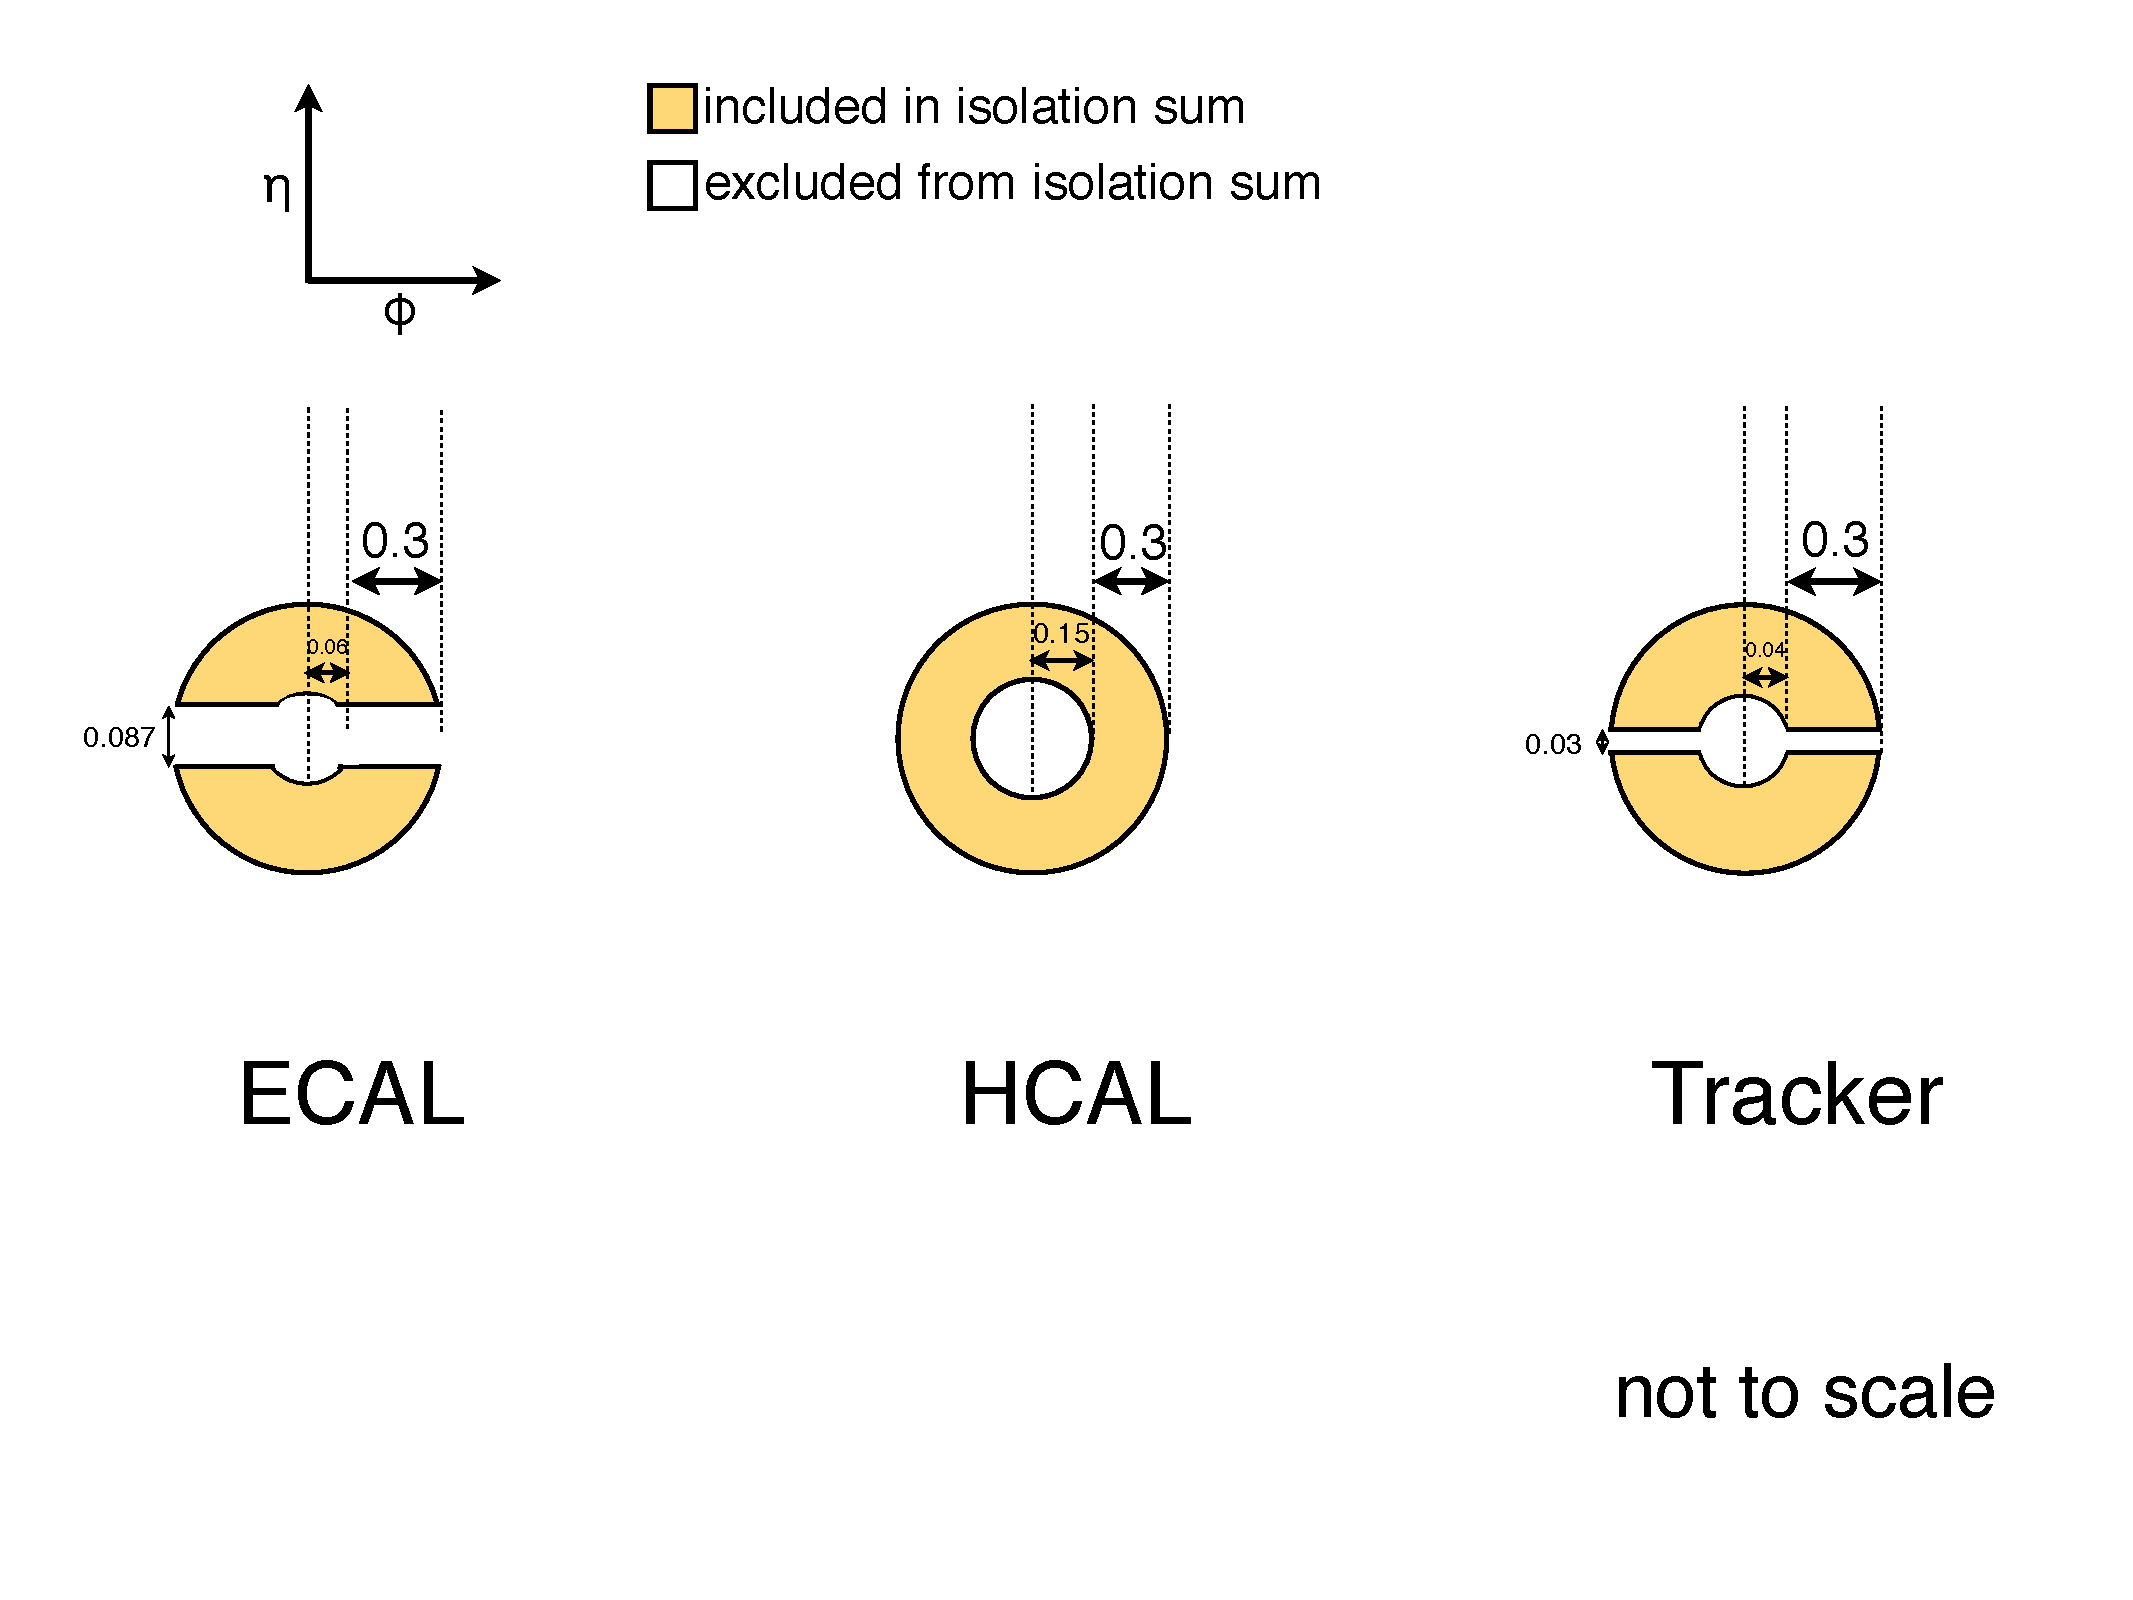
\includegraphics[scale=0.4]{isolation_cones}
	\caption{ECAL, HCAL, and track isolation cones.}
	\label{fig:isolation_cones}
\end{figure}

$\sigma_{i\eta i\eta}$ is the log energy weighted extent of the shower in $\eta$ and is defined as\marginpar{\textcolor{blue}{Added $\sigma_{i\eta i\eta}$ definition}}

\begin{eqnarray}
\sigma_{i\eta i\eta} &=& \frac{\sum_{i = 1}^{25}w_{i}(\eta_{i} - \bar{\eta})^{2}}{\sum_{i = 1}^{25}w_{i}}
\end{eqnarray}
%
where the sums run over the 5 $\times$ 5 matrix of crystals surrounding the seed, $w_{i} = \max(0, 4.7 + \ln(E_{i}/E))$, $E_{i}$ is the energy of the $i^{\mathrm{th}}$ crystal, $E$ is the total energy in the 25 crystals, $\eta_{i}$ is the offset in $\eta$ of the $i^{\mathrm{th}}$ crystal from the seed, and $\bar{\eta}$ is the weighted average $\eta$ of the 25 crystals (using the $w_{i}$ as weights) \cite{CMS-QCD-10-019}.

\marginpar{\textcolor{blue}{Changed average $\rho$; updated fig.~\ref{fig:preselected_rho}}}Figure~\ref{fig:preselected_rho} shows the $\rho$ distribution for a sample of two-photon events, with at least one 40 GeV and one 25 GeV photon, passing the selection requirements in Table~\ref{tab:g_f_criteria} and the trigger requirements in Table~\ref{tab:HLT_by_run_range}.  This sample represents the full 2011 dataset of 4.7 $\mbox{fb}^{-1}$.  Since the average $\rho$ is $\sim 7.5$ GeV, and there is a long tail above this average value, it is necessary to subtract pileup energy from the ECAL and HCAL isolation cones to recover otherwise clean photons in events with large pileup.  The ECAL and HCAL \textit{effective areas} of 0.093 and 0.0281, respectively, are calculated by fitting the average ECAL or HCAL isolation energy vs. $\rho$ in a sample of $Z\rightarrow ee$ events to a straight line.  The slope of the line---which has the units of $\eta\cdot\phi$, or area---is the effective area.

\begin{figure}
	\centering
	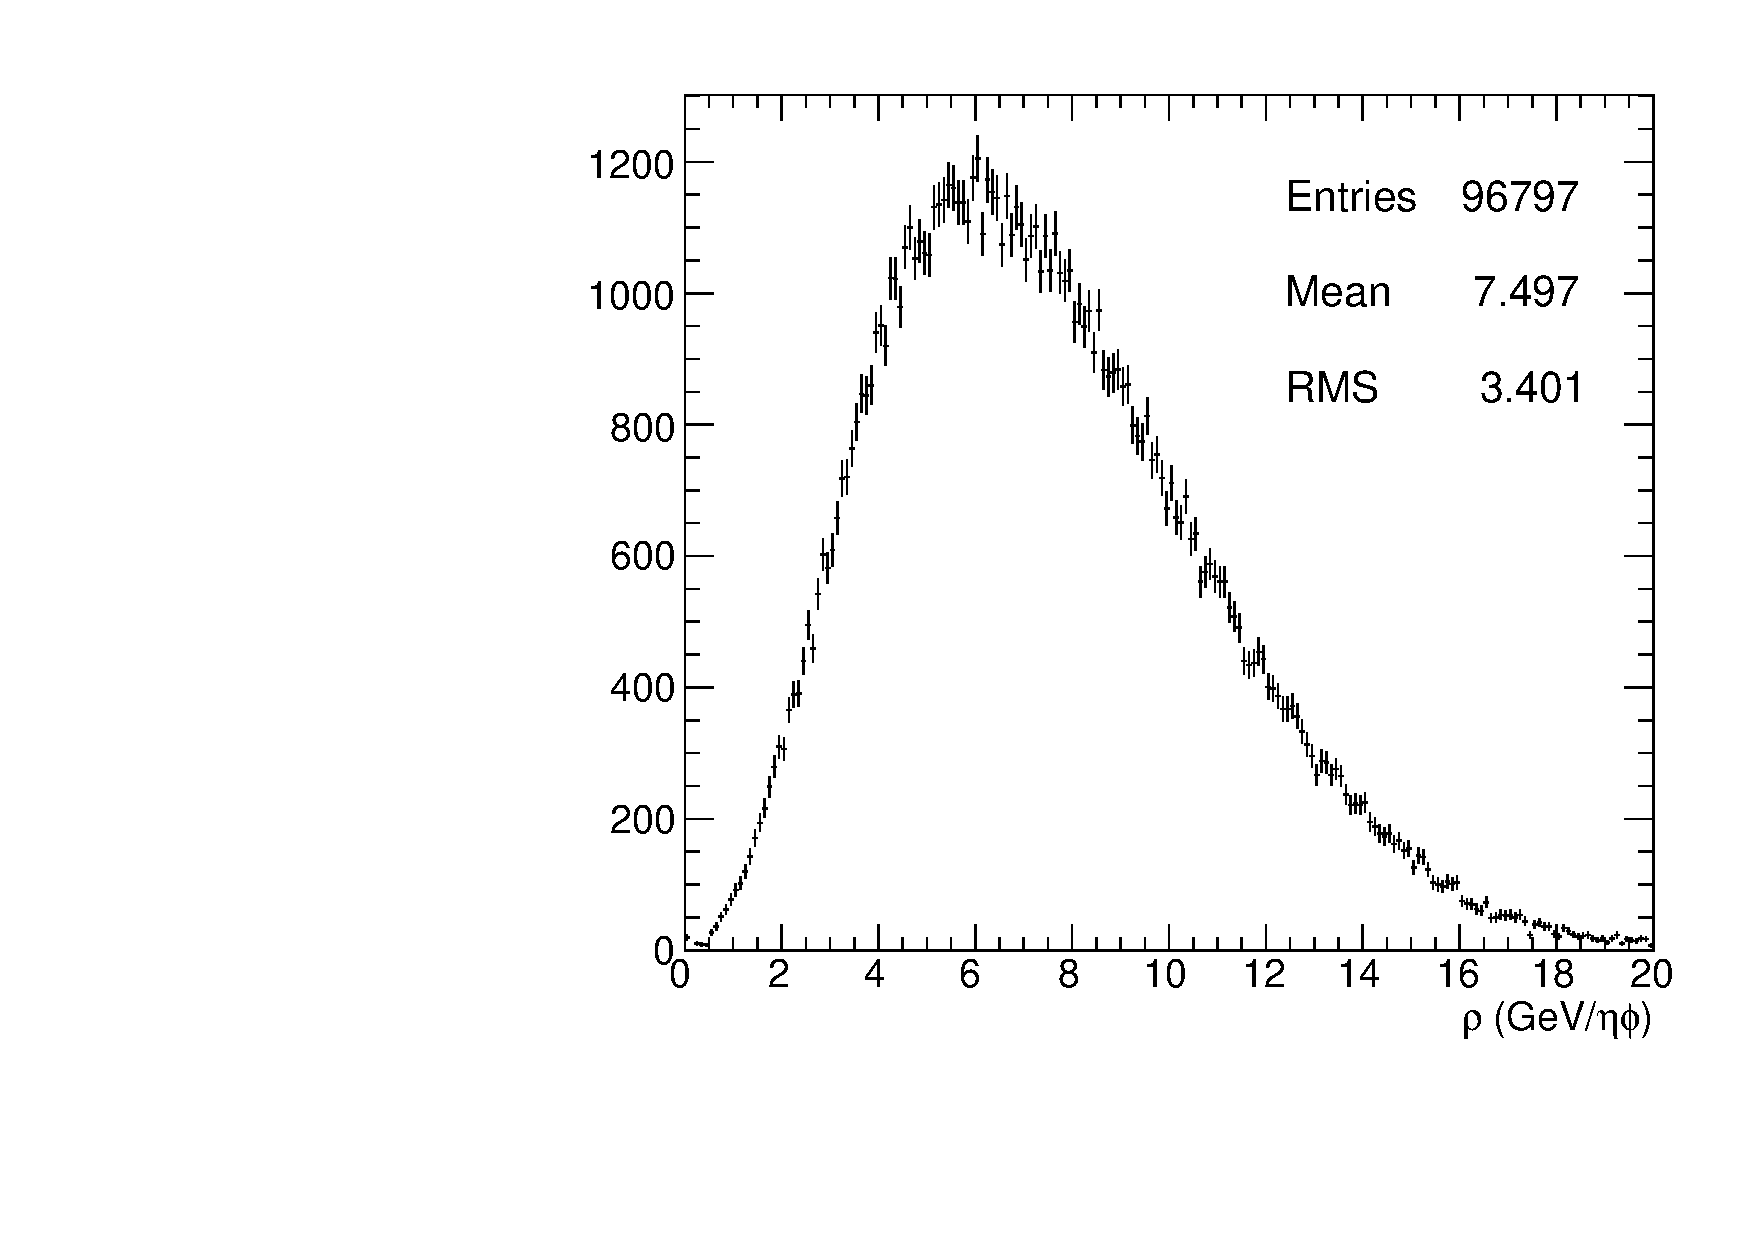
\includegraphics[scale=0.5]{preselected_rho}
	\caption{$\rho$ distribution for a sample of two-photon events, with at least one 40 GeV and one 25 GeV photon, passing the selection requirements in Table~\ref{tab:g_f_criteria} and the trigger requirements in Table~\ref{tab:HLT_by_run_range}.  This sample covers the full 2011 dataset of 4.7 $\mbox{fb}^{-1}$.}
	\label{fig:preselected_rho}
\end{figure}

\marginpar{\textcolor{blue}{New}}The cut on combined isolation of 6 GeV (Table~\ref{tab:g_f_criteria}) is the result of an $S/\sqrt{B}$ optimization procedure \cite{CMS_AN-2011-515}.  $S$ is a sample of photons in simulated GGM events that are products of neutralino decay, while $B$ is a sample of photons matched to generated hadronic jets in simulated QCD events.  Figure~\ref{fig:Icomb_optimization} shows the value of $S/\sqrt{B}$ vs. combined isolation, in particular the pronounced peak around 6 GeV.

\begin{figure}
	\centering
	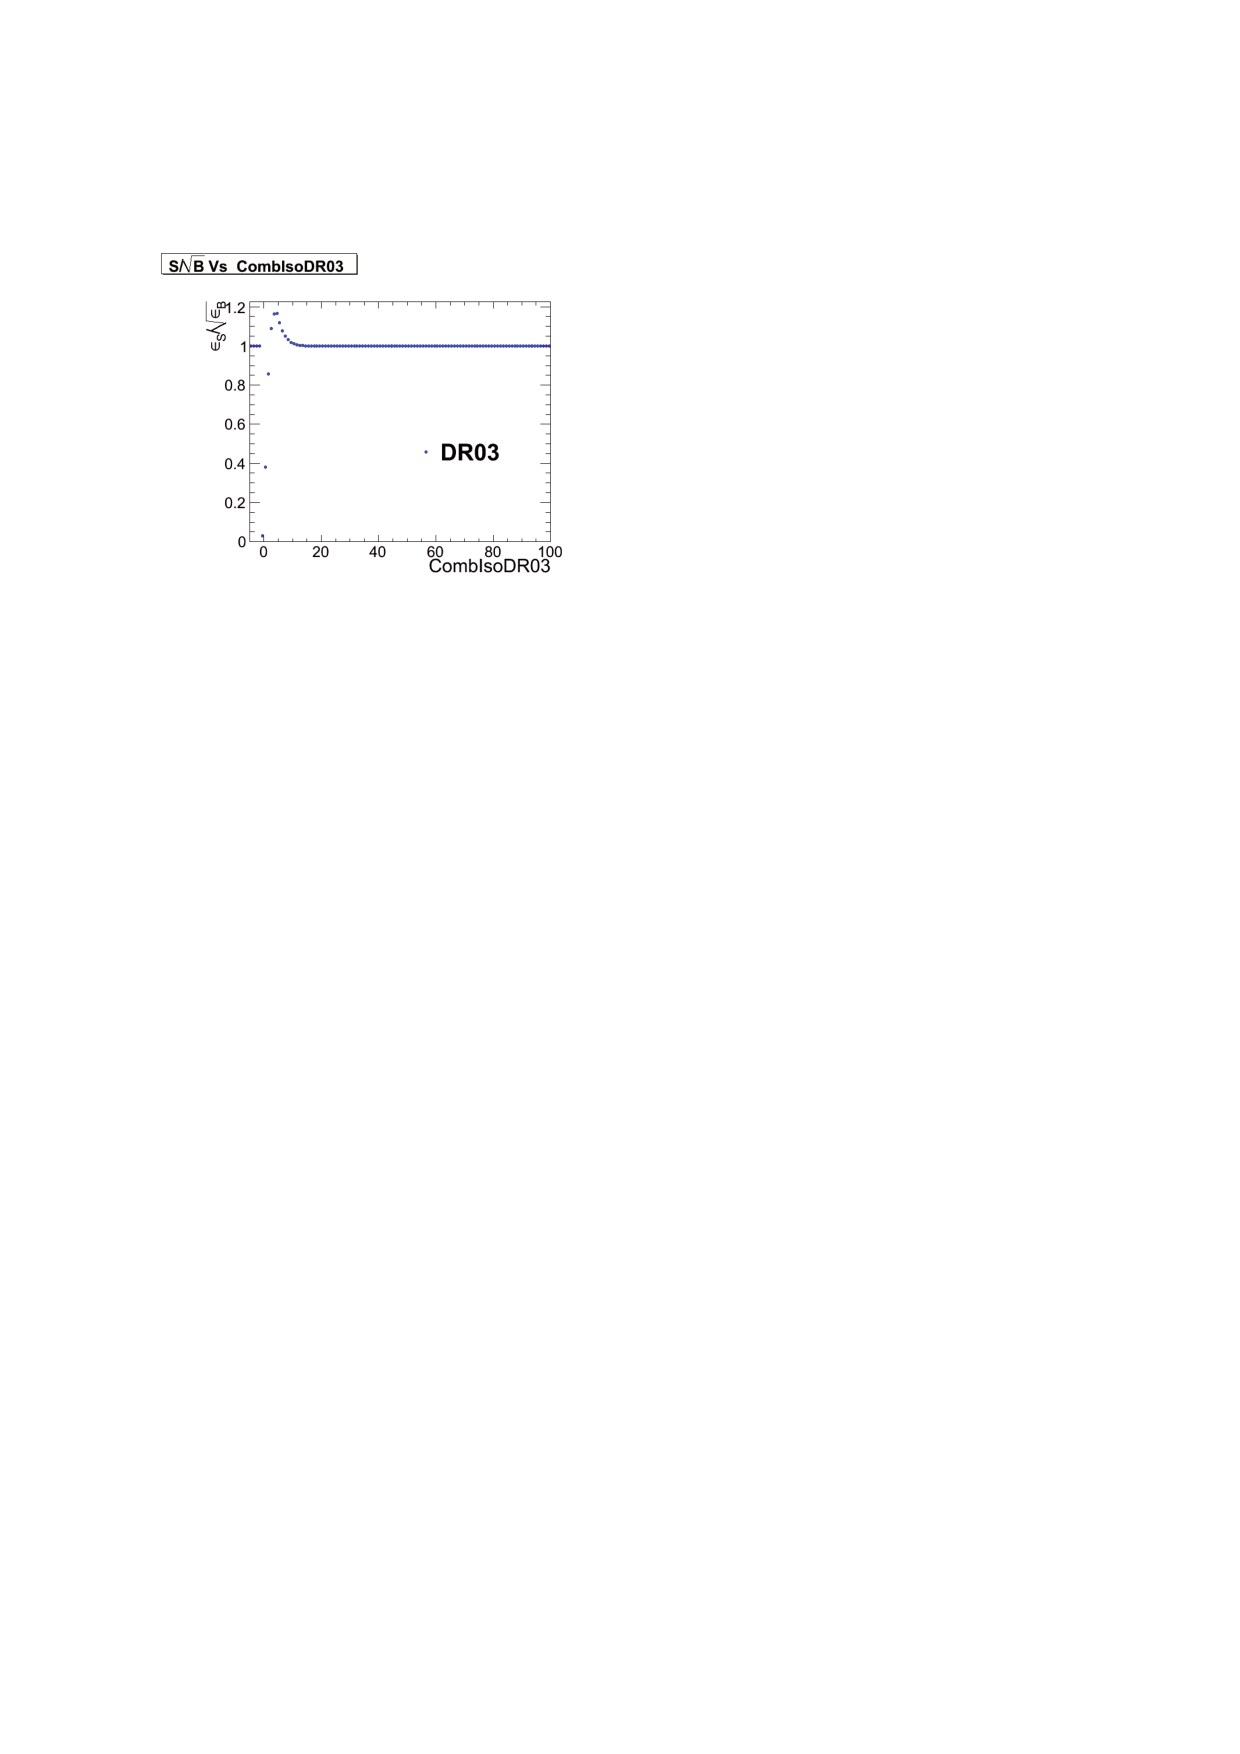
\includegraphics[scale=1.5]{Icomb_optimization}
	\caption{$S/\sqrt{B}$ ($S$ and $B$ defined in the text) vs. $I_{\mathrm{comb}}$.  ``DR03" in the legend indicates that this combined isolation was calculated in $\Delta R = 0.3$ cones, as used throughout this analysis.  Reprinted from Fig. 7 of ref. \cite{CMS_AN-2011-515}.}
	\label{fig:Icomb_optimization}
\end{figure}

The upper bound on fake photon combined isolation guarantees that poorly isolated dijet events, with \MET resolution dissimilar to the candidate diphoton events, do not enter the $\mathit{ff}$ sample.  The exact value of 20 GeV (cf. Table~\ref{tab:g_f_criteria}) arises from a low-\MET $\mathit{ff}$/$\gamma\gamma$ $\chi^{2}$ optimization procedure \cite{CMS_AN-2011-515}.  Figure~\ref{fig:f_comb_iso_upper_bound_optimization} shows the value of the Neyman's $\chi^{2}$ between the $\mathit{ff}$ and $\gamma\gamma$ \MET distributions, truncated at either 25 or 50 GeV, vs. upper bound on fake combined isolation.  As shown in the figure, 20 GeV keeps the $\chi^{2}$ small while also being large enough that a sufficient number of $\mathit{ff}$ events may be collected.

\begin{figure}
	\centering
	\subfloat[Events with $\geq0$ jets.]{\label{fig:f_comb_iso_upper_bound_optimization_geq0j}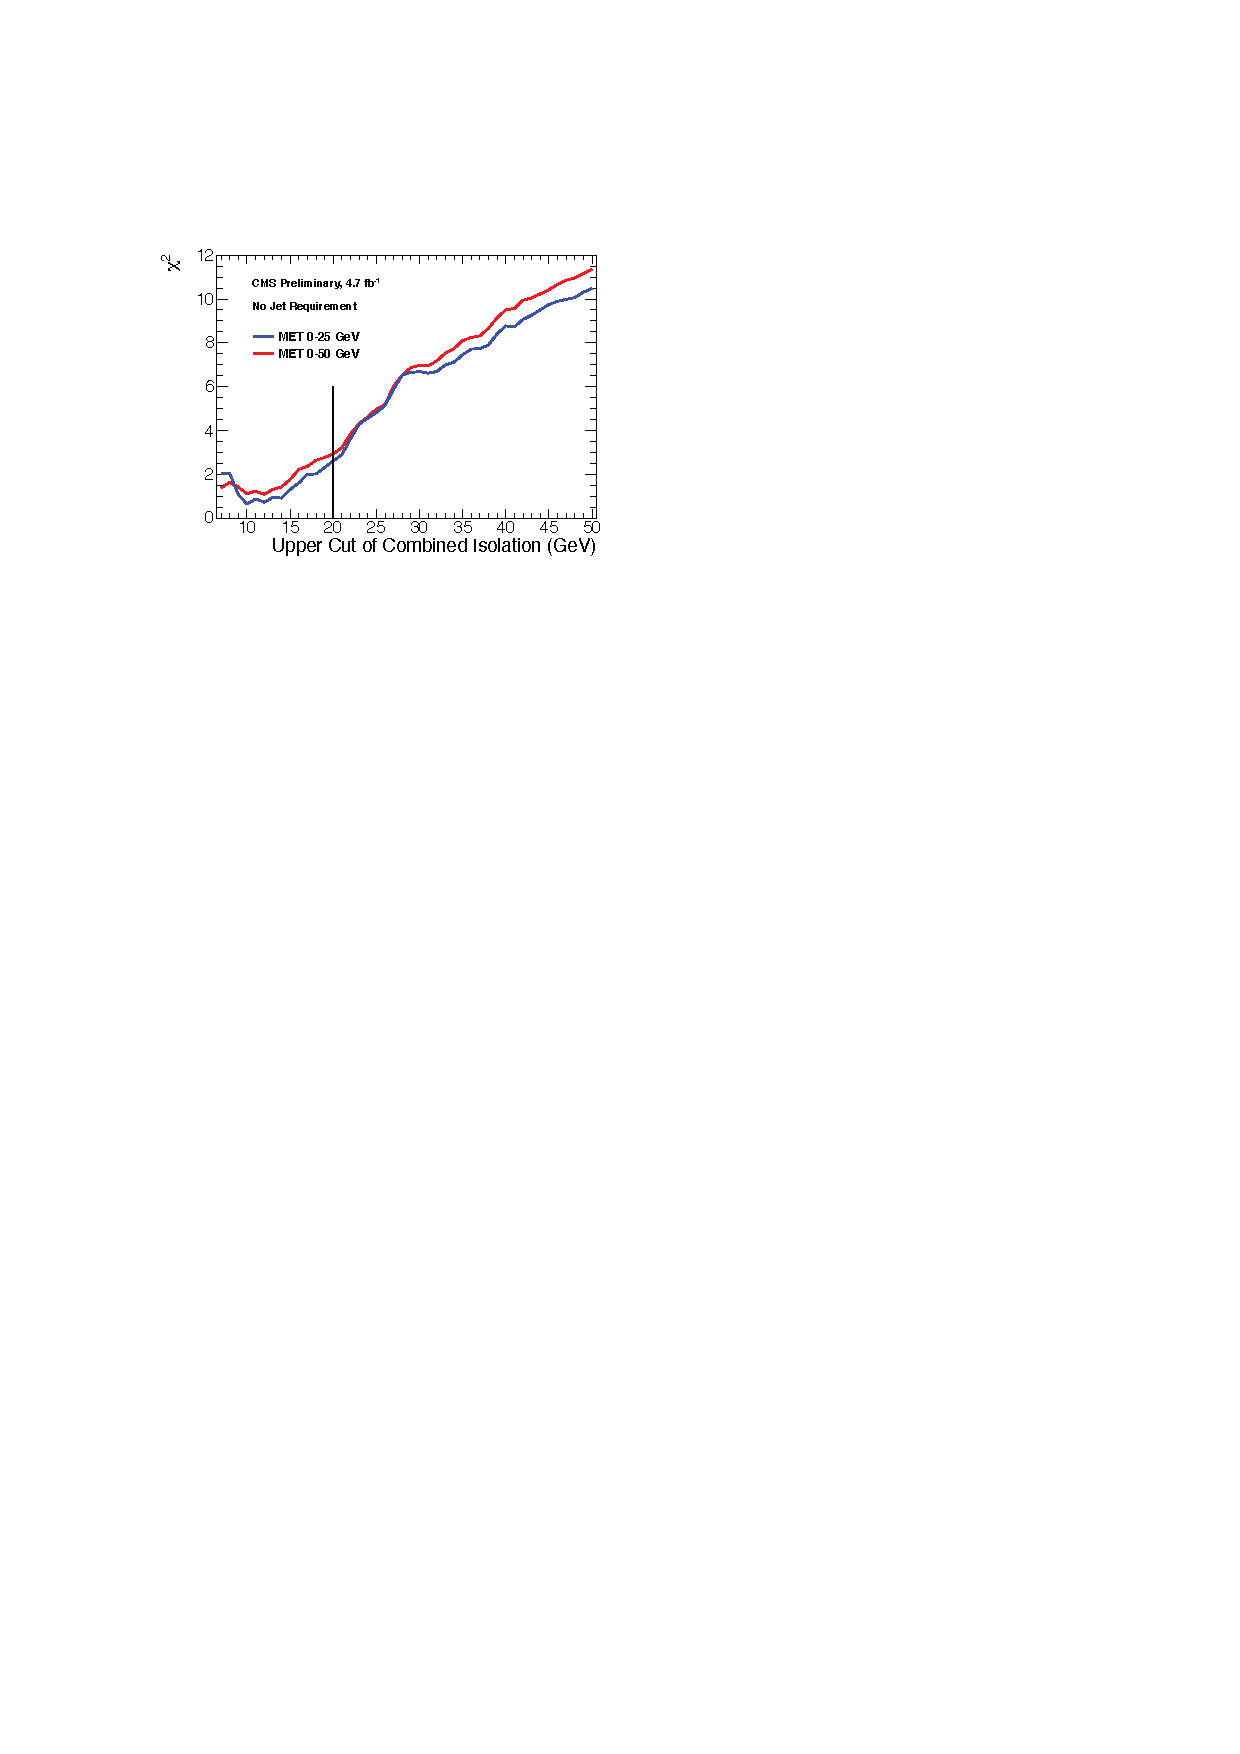
\includegraphics[scale=1.2]{f_comb_iso_upper_bound_optimization_geq0j}}
	\\
	\subfloat[Events with $\geq1$ jet.]{\label{fig:f_comb_iso_upper_bound_optimization_geq1j}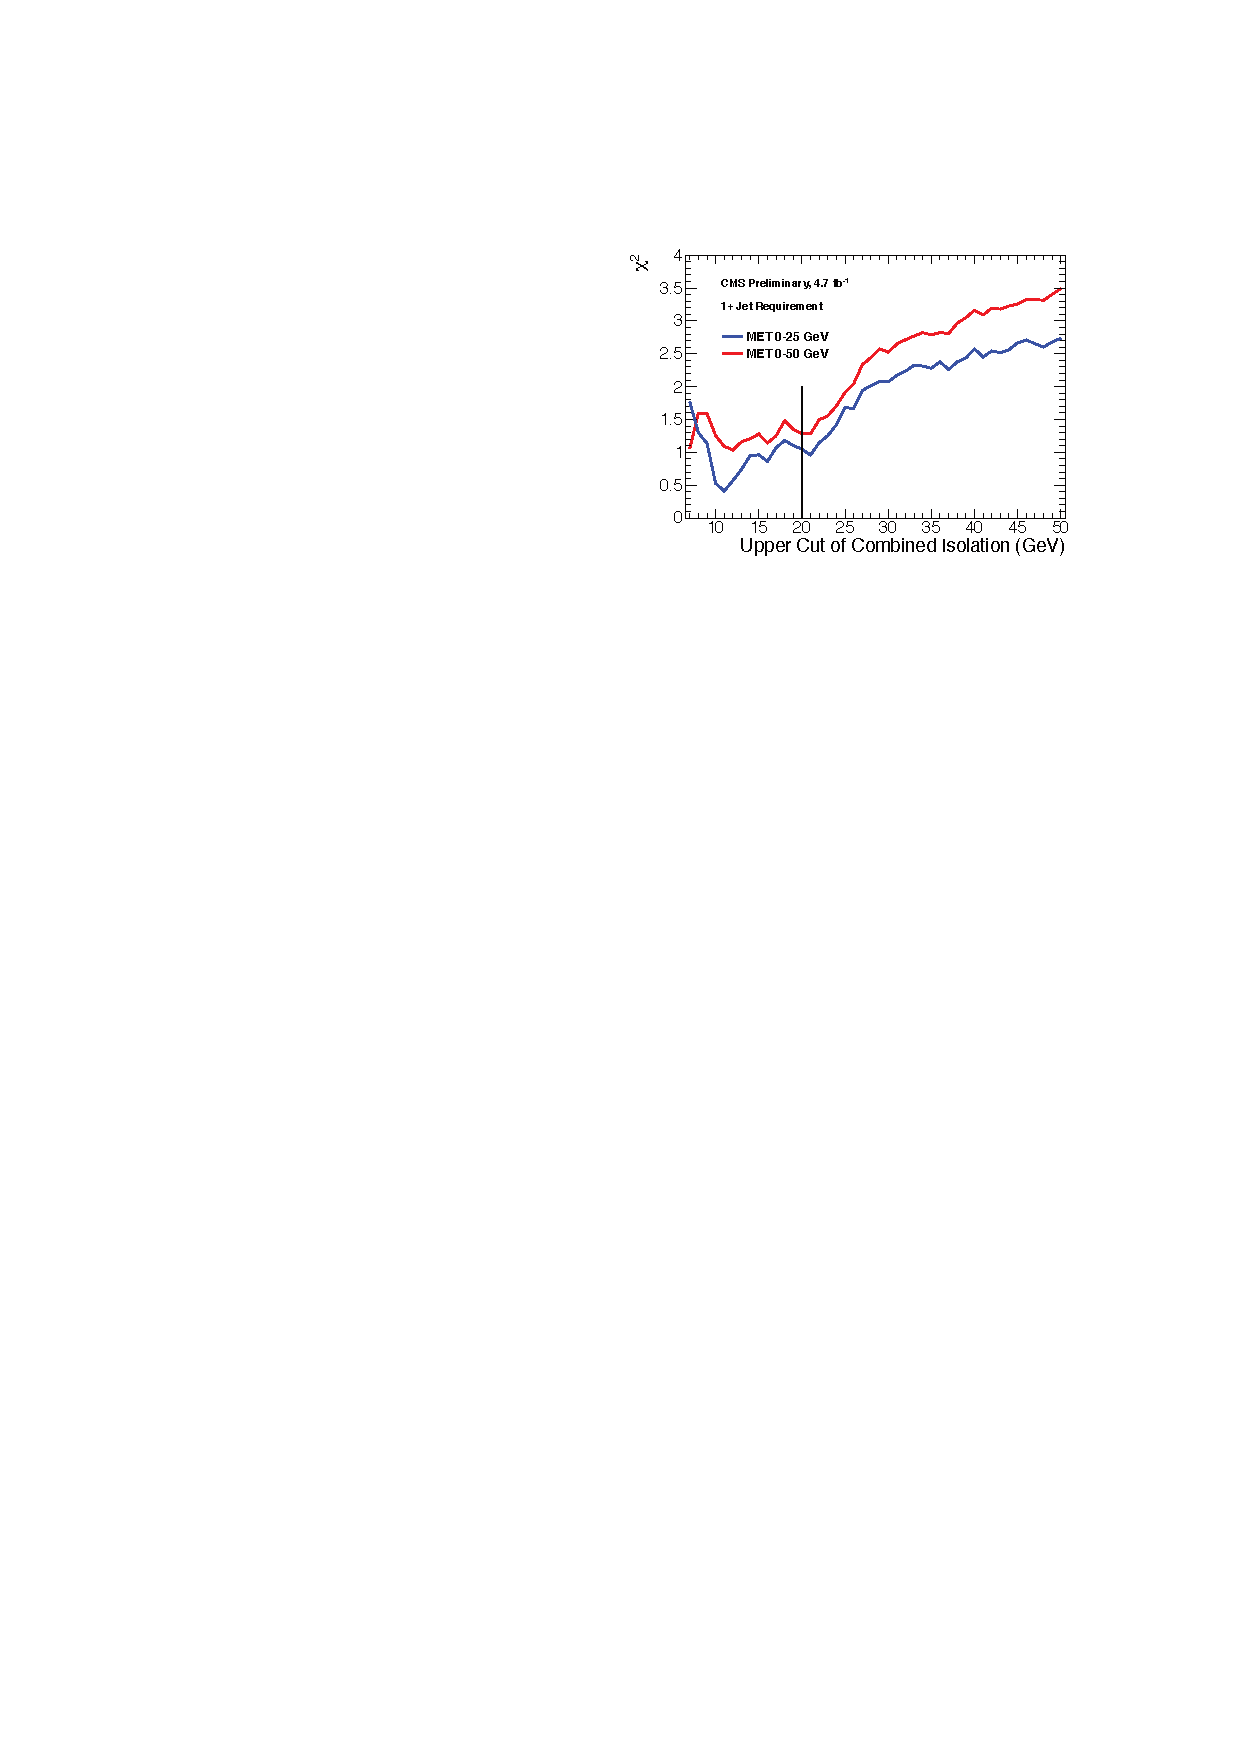
\includegraphics[scale=1.2]{f_comb_iso_upper_bound_optimization_geq1j}}
	\caption{Neyman's $\chi^{2}$ between the $\mathit{ff}$ and $\gamma\gamma$ \MET distributions, truncated at either 25 (red) or 50 (blue) GeV, vs. upper bound on fake combined isolation.  A jet is defined as in Table~\ref{tab:jet_definition_for_Nj_reweighting}, but with the $\Delta R$ cleaning criteria of Table~\ref{tab:jet_definition_for_Nj_reweighting} applied to the two primary EM objects and all additional electrons, photons, and fake photons.  The full reweighting and normalization procedure is employed in the \MET calculation (see Sec.~\ref{sec:Modeling the QCD Background}).  Reprinted from Fig. 9 of ref. \cite{CMS_AN-2011-515}.}
	\label{fig:f_comb_iso_upper_bound_optimization}
\end{figure}

Finally, a ``pixel seed" is defined as a hit in the pixel detector consistent with a track extrapolated from the position of the ECAL SC back to the primary vertex.  Real photons, having no charge and therefore no bending in the magnetic field, should not have a pixel seed.

\subsection{Electrons}
\label{sec:Electrons}

Electrons are reconstructed identically to photons, except that in the electron case the presence of a pixel seed is enforced, rather than vetoed.\footnote{In many CMS analyses, electrons are reconstructed very differently from photons.  In particular, a special tracking algorithm \cite{GSF_reco} is used to best follow a radiating electron.  However, in this analysis, the electron tracking is not used.}  Photons and electrons are defined by very similar criteria so that $Z\rightarrow ee$ events can be used to model the QCD background in the two-photon sample without introducing any bias in the electron energy measurement (cf. Sec.~\ref{sec:Modeling the QCD Background}).

\subsection{Jets and Missing Transverse Energy}
\label{sec:Jets and Missing Transverse Energy}

\subsubsection{Particle Flow}
\label{sec:Particle Flow}

In this analysis, jets and \MET are formed from \textit{particle flow} (PF) candidates.  The particle flow algorithm \cite{PF_algo, PF_perf} uses information from all CMS subdetectors to reconstruct as accurately as possible the positions and momenta of all visible jet constituents, exploiting the fine granularity of the tracker and ECAL to achieve a greatly improved momentum resolution over calorimeter-only jets \cite{CMS_JES_paper}.  The PF algorithm is summarized below \cite{PF_note}.

\begin{enumerate}
\item Reconstruct the fundamental detector objects via iterative procedures
\begin{itemize}
\item Tracks in the inner silicon layers
\begin{itemize}
\item High efficiency and low fake rate for charged hadrons in jets
\item Relaxed primary vertex constraint allows photon conversions, particles originating from nuclear interactions in the silicon, and long-lived particles to be reconstructed
\end{itemize}
\item Calorimeter clusters
\item Muon tracks in the outer muon layers
\end{itemize}
\item Create a ``block" of linked fundamental objects
\begin{itemize}
\item Link silicon tracks to calorimeter clusters via $\Delta R_{\mathrm{track-cluster}}$ (account for electron bremsstrahlung)
\item Link clusters in one calorimeter layer to clusters in a separate layer via $\Delta R_{\mathrm{cluster-cluster}}$
\item Link silicon tracks to muon tracks via global track $\chi^{2}$
\end{itemize}
\item ID the particles in the block
\begin{itemize}
\item If global (silicon + muon layers) muon $p_{T}$ is compatible with silicon track $p_{T}$, ID as a muon and remove corresponding tracks from block
\item ID electron tracks via special algorithm and removed all corresponding tracks and cluster from block
\item Remove fake tracks from the block
\item Allow multiple tracks to be associated to one HCAL cluster, but not multiple HCAL clusters to be associated to one track---for each track, keep only the HCAL cluster link that is closest in $\Delta R$ to the track
\item If the cluster energy is significantly larger then the energy of the linked tracks, ID as a PF photon or PF neutral hadron
\item If the cluster is not linked to a track, ID as a PF photon or PF neutral hadron
\item If the cluster energy is smaller than the energy of the linked tracks, ID each track as a PF charged hadron
\end{itemize}
\end{enumerate}

\subsubsection{Jets}
\label{sec:Jets}

PF candidates are clustered into jets by means of the anti-$k_{T}$ algorithm with $R = 0.5$ \cite{AK5}.  In this algorithm, all possible pairs of PF candidates $i, j$ are looped over, and the pairs that minimize the distance variable

\begin{eqnarray}
d_{ij} = \frac{\Delta R_{ij}^{2}}{R^{2}\max(k_{Ti}^{2}, k_{Tj}^{2})}
\end{eqnarray}
%
are clustered together, where $k_{Ti}$ is the transverse momentum of PF candidate $i$.  The process is repeated, using the pairwise-clustered PF candidates as input objects to the next round of clustering, until $d_{ij} > 1/k_{Ti}^{2}$ for all pairs of clustered PF candidates \cite{Salam_talk}.  An illustration is given in Figure~\ref{fig:anti-kT}.  \marginpar{\textcolor{blue}{Added reference to Fig.~\ref{fig:anti-kT}}}The anti-$k_{T}$ algorithm is infrared and collinear safe, leading to well-behaved theoretical predictions and ease of comparison between data and MC simulation.  It also tends to form circular jets, making it easy for experimental effects such as expected out-of-cone energy and fiducial acceptance to be measured or simulated.  For these reasons, the anti-$k_{T}$ jet clustering algorithm was chosen for this analysis.

\begin{figure}
	\centering
	\includegraphics[scale=1.5]{anti-kT}
	\caption{Example event display showing jets clustered via the anti-$k_{T}$ algorithm.  y is pseudorapidity.  Reprinted from slide 85 of ref. \cite{Salam_talk}.}
	\label{fig:anti-kT}
\end{figure}

Once jets are found, they must be corrected for biases in the energy measurement due to non-compensation \cite{Wigmans}, invisible energy (lost to overcoming nuclear binding energy, in neutrinos, or in unclustered muons, for example) \cite{Wigmans}, detector geometry and cracks \cite{CDF_JEC_website}, zero suppression and trigger inefficiencies \cite{CMS_MET_paper}, pileup, and effects of the clustering algorithm \cite{CDF_JEC_website}.  Four multiplicative correction factors are applied to the raw jet four-momentum $p_{\mu}^{\mathrm{raw}}$ \cite{CMS_JES_paper}:

\begin{itemize}
\item $C_{\mathrm{offset}}(p_{T}^{\mathrm{raw}})$, which accounts for extra energy due to noise, pileup, and the underlying event;
\item $C_{\mathrm{MC}}(C_{\mathrm{offset}}p_{T}^{\mathrm{raw}}, \eta)$, which is derived from MC and accounts for most of the $p_{T}$ and $\eta$ dependence;
\item $C_{\mathrm{rel}}(\eta)$, which accounts for the remaining differences in uniformity over the entire calorimeter between data and MC; and
\item $C_{\mathrm{abs}}(C_{\mathrm{rel}}C_{\mathrm{MC}}C_{\mathrm{offset}}p_{T}^{\mathrm{raw}})$, which accounts for the remaining differences in linearity over the full $p_{T}$ range between data and MC.
\end{itemize}

Figure~\ref{fig:total_JEC} shows the total jet energy correction factor $C_{\mathrm{offset}}C_{\mathrm{MC}}C_{\mathrm{rel}}C_{\mathrm{abs}}$ vs. $\eta$ for jets reconstructed with the anti-$k_{T}$ algorithm, $R = 0.5$.  The PF jet corrections are more uniform across $\eta$ than those of CALO jets (composed of simple calorimeter towers) or JPT jets (Jet Plus Tracks; composed of calorimeter energies replaced, where possible, with matching track $p_{T}$) \cite{JPT}.  In addition, for $p_{T}$ in the range 30-200 GeV and $|\eta|$ up to 2.0, the PF jet energy correction uncertainty is lower than that of the other two types of jets, and never exceeds $\sim$ 3\% \cite{CMS_JES_paper}.  The superior performance of PF jets motivates their use in this search.

\begin{figure}
	\centering
	\subfloat[Jet $p_{T} = 50$ GeV.]{\label{fig:total_JEC_50_GeV}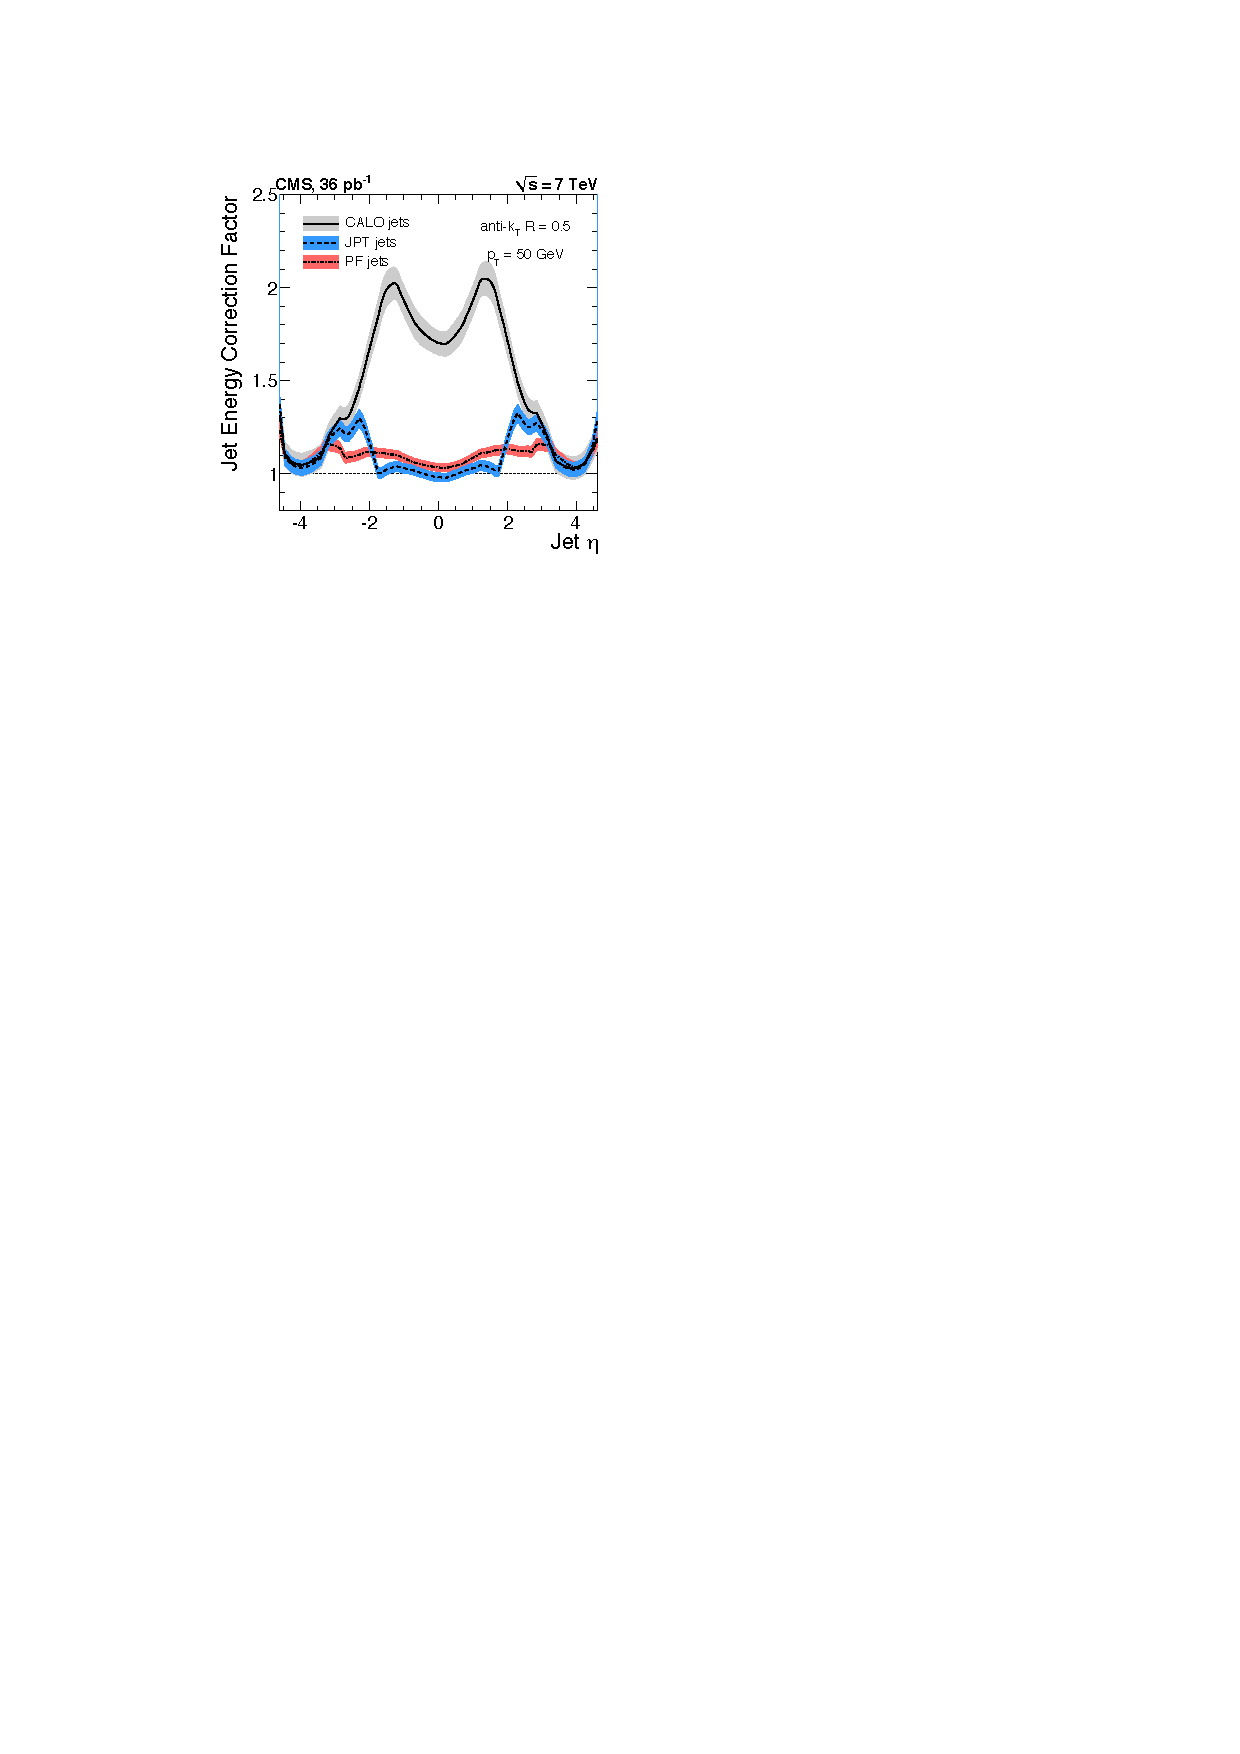
\includegraphics[scale=1.0]{total_JEC_50_GeV}}
	\hspace{1cm}
	\subfloat[Jet $p_{T} = 200$ GeV.]{\label{fig:total_JEC_50_GeV}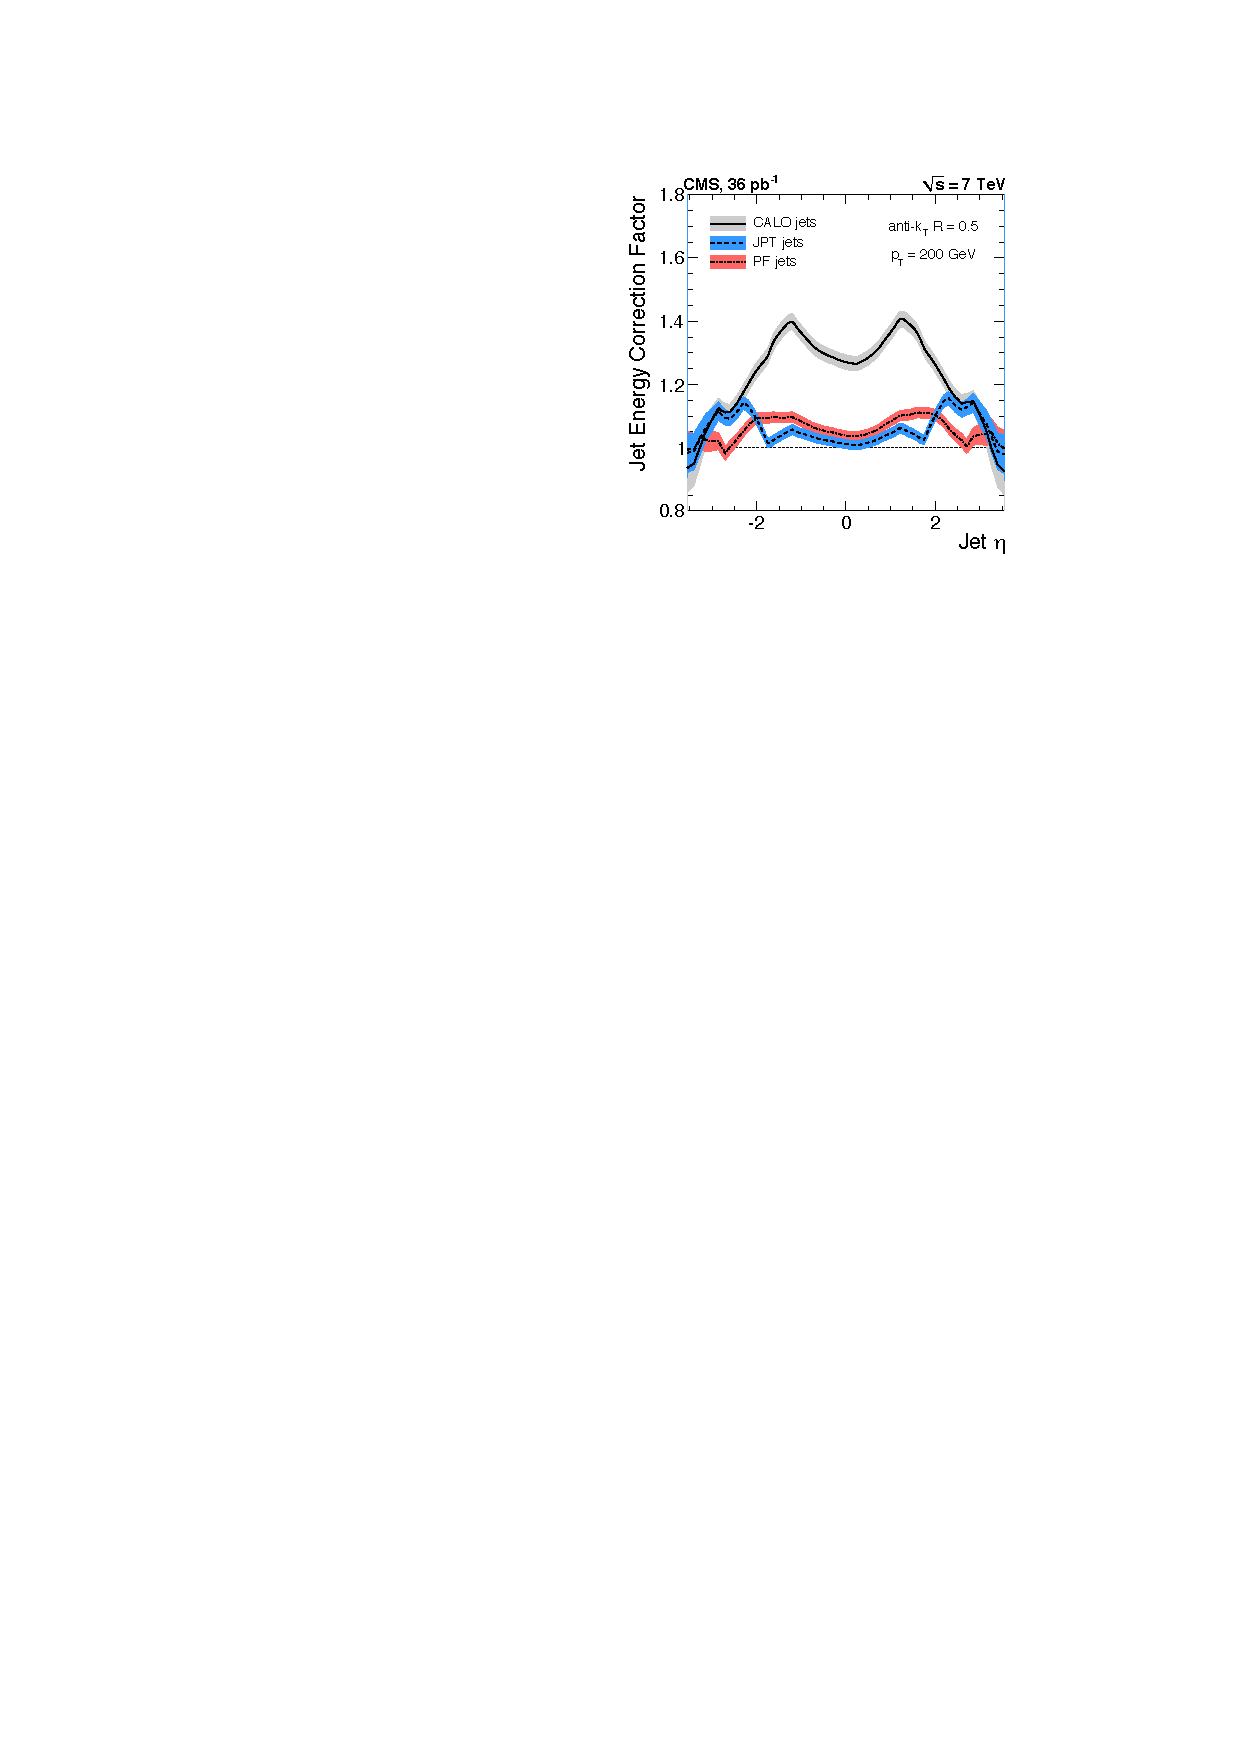
\includegraphics[scale=1.0]{total_JEC_200_GeV}}
	\caption{Total jet energy correction factor $C_{\mathrm{offset}}C_{\mathrm{MC}}C_{\mathrm{rel}}C_{\mathrm{abs}}$ vs. $\eta$, including uncertainty band, for jets reconstructed with the anti-$k_{T}$ algorithm, $R = 0.5$.  Reprinted from Fig. 26 of ref. \cite{CMS_JES_paper}.}
	\label{fig:total_JEC}
\end{figure}

In this analysis, candidate and QCD control events are binned by number of jets satisfying the criteria in Table~\ref{tab:jet_definition_for_Nj_reweighting}.

\begin{table}[hcbp]
\caption{Definition of HB/HE hadronic jets.}
\centering
\begin{minipage}{\textwidth}
\centering
\begin{tabular}{|c|c|}
\hline
Variable & Cut \\
\hline
\hline
Algorithm & \verb+L1FastL2L3Residual+ corrected PF \\
\hline
$p_{T}$ & $> 30$ GeV \\
\hline
$|\eta|$ & $< 2.6$ \\
\hline
\begin{tabular}[c]{@{}c@{}}Neutral hadronic\\energy fraction\end{tabular} & $< 0.99$ \\
\hline
\begin{tabular}[c]{@{}c@{}}Neutral electromagnetic\\energy fraction\end{tabular} & $< 0.99$ \\
\hline
Number of constituents & $> 1$ \\
\hline
Charged hadronic energy & $> 0.0$ GeV if $|\eta|  < 2.4$ \\
\hline
Number of charged hadrons & $> 0$ if $|\eta|  < 2.4$ \\
\hline
\begin{tabular}[c]{@{}c@{}}Charged electromagnetic\\energy fraction\end{tabular} & $< 0.99$ if $|\eta| < 2.4$ \\
\hline
\begin{tabular}[c]{@{}c@{}}$\Delta R$ to nearest PF electron\footnote{A PF electron is defined as an electron reconstructed with the PF algorithm \cite{CMS_AN-2010/034} with $p_{T} >$ 15 GeV, $|\eta| <$ 2.6, and ($I_{\mathrm{charged}} + I_{\mathrm{photon}} + I_{\mathrm{neutral}}$)/$p_{T} <$ 0.2, where $I_{\mathrm{charged}}$($I_{\mathrm{photon}}$)($I_{\mathrm{neutral}}$) is the sum of PF charged hadron(PF photon)(PF neutral hadron) momenta in a $\Delta$R = 0.4 cone around the PF electron.}, muon\footnote{Muons are reconstructed \cite{CMS_CR-2009/347} from a combination of muon station and inner tracker hits.  Here, a muon must have track $\chi^{2} <$ 10, at least one good muon station hit, inner track transverse impact parameter $<$ 0.02 cm, inner track longitudinal impact parameter $<$ 0.5 cm, $p_{T} >$ 15 GeV, $|\eta| <$ 2.6, and ($I_{\mathrm{ECAL}} + I_{\mathrm{HCAL}} + I_{\mathrm{track}}$)/$p_{T} <$ 0.2, where $I_{\mathrm{ECAL}}$($I_{\mathrm{HCAL}}$)($I_{\mathrm{track}}$) is the sum of ECAL(HCAL)(track) momenta in a $\Delta$R = 0.3 cone around the muon.},\\or one of the two\\primary EM objects\end{tabular} & $> 0.5$ \\
\hline
\end{tabular}
\end{minipage}
\label{tab:jet_definition_for_Nj_reweighting}
\end{table}

\subsubsection{Missing Transverse Energy}
\label{sec:MET}

To be consistent with the jet reconstruction, \MET in this analysis is also reconstructed from PF candidates.  Raw \MET is defined as

\begin{eqnarray}
\not\!\! E_{T\mathrm{raw}} &=& |-\sum_{i = 1}^{n_{\mathrm{PF}}}\overrightarrow{p}_{Ti}|
\end{eqnarray}
%
where $n_{\mathrm{PF}}$ is the number of PF candidates in the event.  $\not\!\! E_{T\mathrm{raw}}$ may be corrected for the same effects that necessitate jet corrections, since $\not\!\! E_{T\mathrm{raw}}$ is usually the result of jet mis-measurement (except, of course, in electroweak physics processes that include an energetic neutrino, or SUSY production).  CMS \textit{Type-I} \MET corrections simply involve replacing the PF jets with their corrected energies (cf. Sec~\ref{sec:Jets}) and recalculating \MET.  Only jets with electromagnetic fraction (EMF) below 90\% and $p_{T} > 20$ GeV are replaced.  \marginpar{\textcolor{blue}{Removed italics in ``electromagnetic fraction"}}This ensures that very electromagnetic jets (as well as isolated leptons, which also receive no correction), which consist chiefly of neutral pions and are measured accurately by the ECAL, do not receive a correction derived for jets with a large fraction of their energy in charged hadrons.  In addition, the $p_{T}$ cut guarantees that jet corrections are only applied where they are known to within a few percent.  For this search, the level of agreement between the SM background estimate and the two-photon search sample in a low-\MET control region is the same regardless of whether the \MET is corrected or not, so for simplicity the Type-I \MET corrections are not used (see Sec.~\ref{sec:Errors on the Background Prediction}).

Figure~\ref{fig:MET_resolution} shows the $\sigma$ of a Gaussian fit to the x- and y-components of calibrated \MET vs. the calibrated PF $E_{T}$ sum in a sample of events containing at least two jets with $p_{T} > 25$ GeV.  Again, PF \MET outperforms \MET constructed of calorimeter towers or track-corrected calorimeter deposits.

\begin{figure}
	\centering
	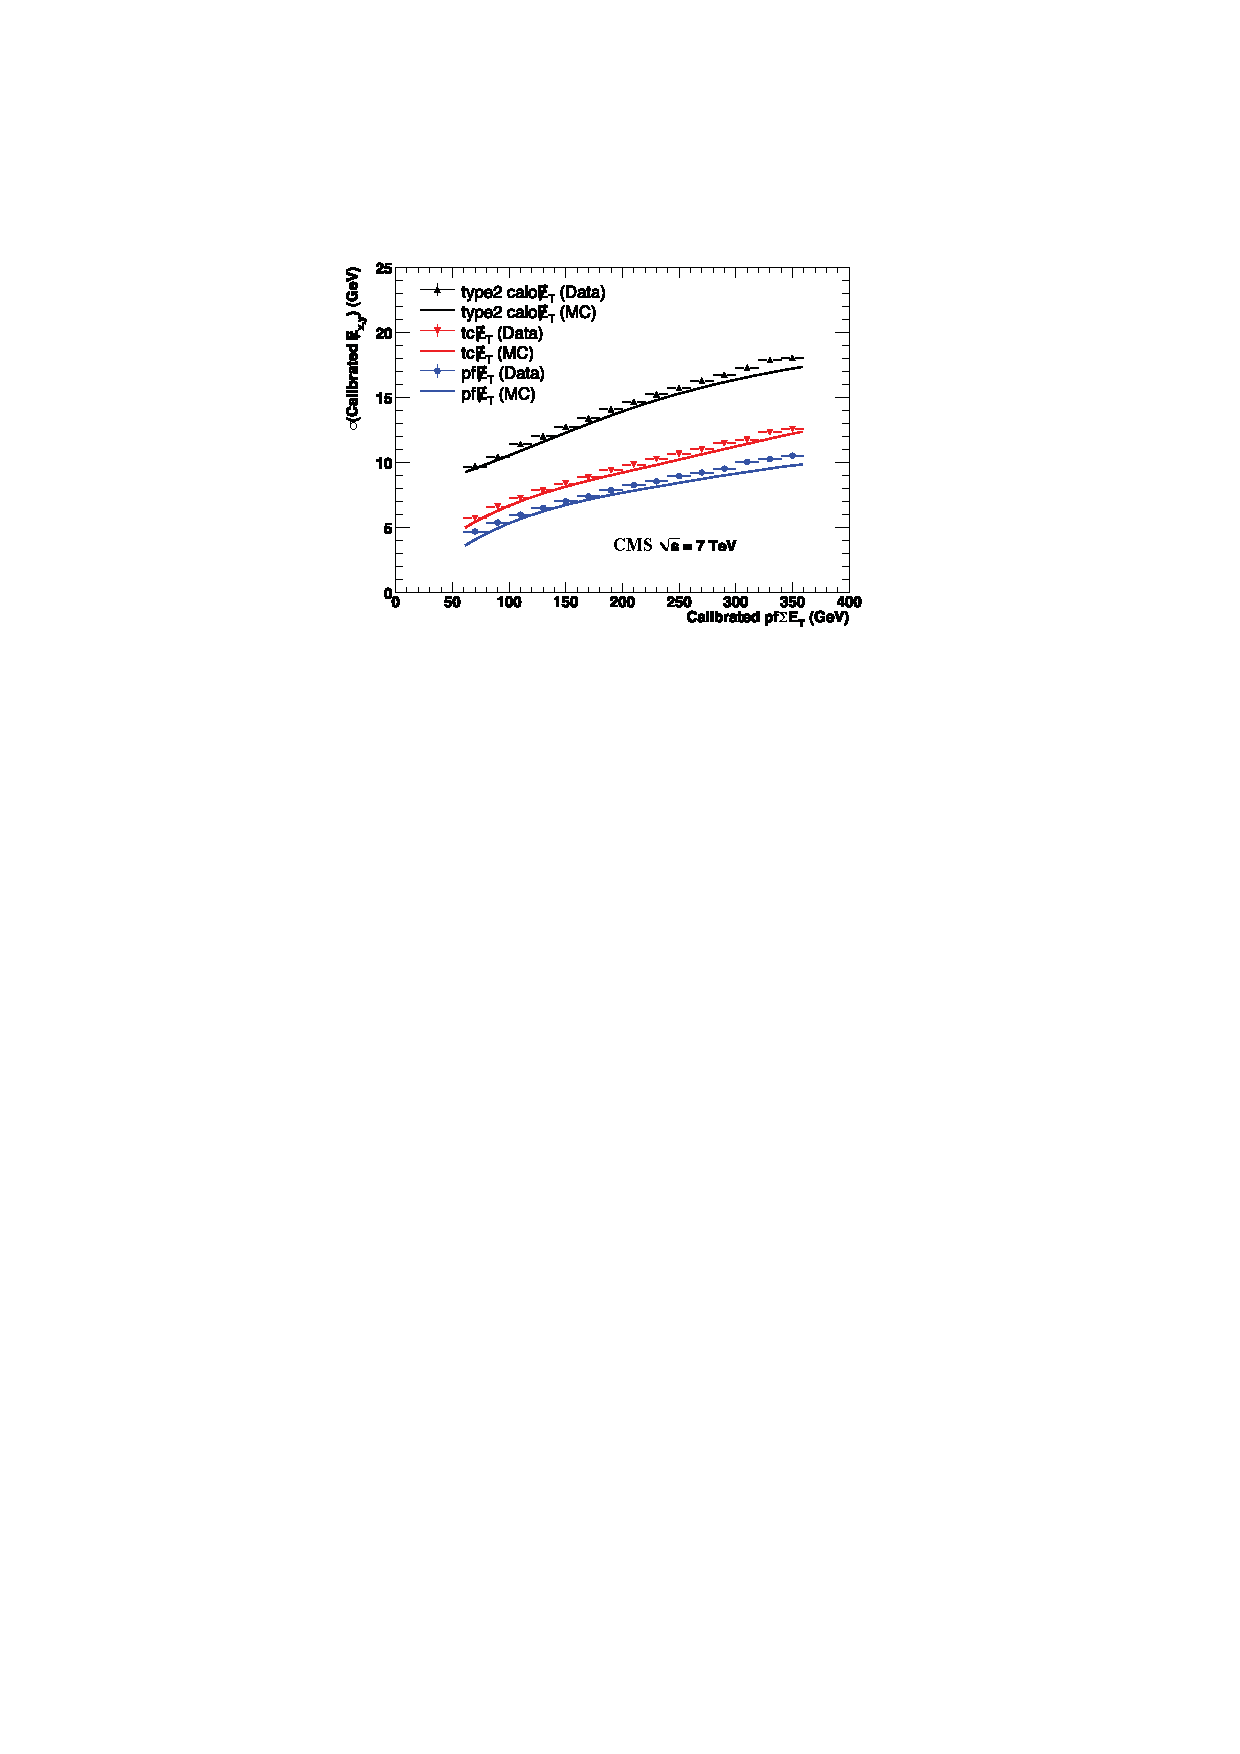
\includegraphics[scale=1.0]{MET_resolution}
	\caption{$\sigma$ of a Gaussian fit to the x- and y-components of calibrated \MET vs. the calibrated PF $E_{T}$ sum in a sample of events containing at least two jets with $p_{T} > 25$ GeV.  $\sigma$ is calibrated such that the \MET scale is equal for all three algorithms.  PF $\sum E_{T}$ is corrected, on average, to the particle level using a Pythia v8 simulation \cite{Pythia8}.  The blue markers (data) and line (MC) refer to PF jets.  Reprinted from Fig. 13 of ref. \cite{CMS_MET_paper}.}
	\label{fig:MET_resolution}
\end{figure}

\section{HLT}
\label{sec:HLT}

From the objects described in Sec.~\ref{sec:Object Reconstruction}, four samples of events are formed:

\begin{itemize}
\item $\gamma\gamma$ candidate sample, in which the two highest $E_{T}$ objects are photons,
\item $e\gamma$ control sample, in which the two highest $E_{T}$ objects are one electron and one photon,
\item $ee$ control sample, in which the two highest $E_{T}$ objects are electrons, and
\item $\mathit{ff}$ control sample, in which the two highest $E_{T}$ objects are fakes.
\end{itemize}
%
In all samples, the leading EM object is required to have offline reconstructed $E_{T} > 40$ GeV, while the trailing EM object is required to have offline reconstructed $E_{T} > 25$ GeV.  The high level triggers used to select the four samples, by run range, are listed in Table~\ref{tab:HLT_by_run_range}.  No trigger is prescaled.

\begin{table}[hcbp]
\caption{HLT paths triggered by the $\gamma\gamma\mbox{, }e\gamma\mbox{, }ee\mbox{, and }\mathit{ff}$ samples, by run range.  No triggers are prescaled.}
\centering
\begin{tabular}{|c|m{2.6cm}|m{2.6cm}|m{2.6cm}|m{2.6cm}|}
\hline
Run range & $\gamma\gamma$ & $e\gamma$ & $ee$ & $\mathit{ff}$ \\
\hline
\hline
160404-163261 & \texttt{Photon26\_}\newline \texttt{IsoVL\_}\newline \texttt{Photon18} & \texttt{Photon26\_}\newline \texttt{IsoVL\_}\newline \texttt{Photon18} & \texttt{Photon26\_}\newline \texttt{IsoVL\_}\newline \texttt{Photon18} & \texttt{Photon26\_}\newline \texttt{IsoVL\_}\newline \texttt{Photon18} \\
\hline
161216-166967 & \texttt{Photon36\_}\newline \texttt{CaloIdL\_}\newline \texttt{Photon22\_}\newline \texttt{CaloIdL} & \texttt{Photon36\_}\newline \texttt{CaloIdL\_}\newline \texttt{Photon22\_}\newline \texttt{CaloIdL} & \texttt{Photon36\_}\newline \texttt{CaloIdL\_}\newline \texttt{Photon22\_}\newline \texttt{CaloIdL} & \texttt{Photon36\_}\newline \texttt{CaloIdL\_}\newline \texttt{Photon22\_}\newline \texttt{CaloIdL} \\
\hline
166347-180252 & \texttt{Photon36\_}\newline \texttt{CaloIdL\_}\newline \texttt{IsoVL\_}\newline \texttt{Photon22\_}\newline \texttt{CaloIdL\_}\newline \texttt{IsoVL} & \texttt{Photon36\_}\newline \texttt{CaloIdL\_}\newline \texttt{IsoVL\_}\newline \texttt{Photon22\_}\newline \texttt{CaloIdL\_}\newline \texttt{IsoVL} & \texttt{Photon36\_}\newline \texttt{CaloIdL\_}\newline \texttt{IsoVL\_}\newline \texttt{Photon22\_}\newline \texttt{CaloIdL\_}\newline \texttt{IsoVL} & \texttt{Photon36\_}\newline \texttt{CaloIdL\_}\newline \texttt{IsoVL\_}\newline \texttt{Photon22\_}\newline \texttt{CaloIdL\_}\newline \texttt{IsoVL}\newline\newline \texttt{Photon36\_}\newline \texttt{CaloIdL\_}\newline \texttt{IsoVL\_}\newline \texttt{Photon22\_}\newline \texttt{R9Id}\newline\newline \texttt{Photon36\_}\newline \texttt{R9Id\_}\newline \texttt{Photon22\_}\newline \texttt{CaloIdL\_}\newline \texttt{IsoVL}\newline\newline \texttt{Photon36\_}\newline \texttt{R9Id\_}\newline \texttt{Photon22\_}\newline \texttt{R9Id} \\
\hline
\end{tabular}
\label{tab:HLT_by_run_range}
\end{table}

Each piece of the HLT path name is defined as follows.

\begin{itemize}
\item \verb+Photon+: Energy deposit in the ECAL that fired an L1 trigger (cf. Sec.~\ref{sec:Level 1 and High Level Trigger Systems}).  For \marginpar{\textcolor{blue}{Switched HLT path names to verbatim font and added reference to L1 section}}\verb+Photon26_IsoVL_Photon18+, the L1 seed $E_{T}$ threshold is 12 GeV, while for all other triggers in Table~\ref{tab:HLT_by_run_range} it is 20 GeV (cf. Sec.~\ref{sec:Level 1 and High Level Trigger Systems}).
\item Integer following the word \verb+Photon+: $E_{T}$ threshold in GeV for offline reconstructed photon, using the full photon reconstruction of Sec.~\ref{sec:Photons} minus the laser calibrations and assuming the primary vertex at (0, 0, 0).
\item \verb+CaloIdL+: For EB photons, $H/E < 0.15$ and $\sigma_{i\eta i\eta} < 0.014$.
\item \verb+IsoVL+: $I_{\mathrm{ECAL}} < 0.012E_{T} + 6$ GeV, $I_{\mathrm{HCAL}} < 0.005E_{T} + 4$ GeV, and $I_{\mathrm{track}} < 0.002E_{T} + 4$ GeV.
\item \verb+R9Id+: $R9 > 0.8$.
\end{itemize}
%
In addition, the versions of \marginpar{\textcolor{blue}{Switched HLT path names to verbatim font}}\verb+HLT_Photon26_IsoVL_Photon18+ and \\\verb+Photon36_CaloIdL_Photon22_CaloIdL+ that were active during runs 160404-163268 included a cut $E_{\mathrm{max}}/E_{5\times 5} < 0.98$ for spike rejection.  $E_{\mathrm{max}}$ is the energy in the highest energy crystal of the EM cluster and $E_{5\times 5}$ is the energy in the 5$\times$5 crystal matrix around the seed crystal.  For runs after 163268, Swiss cross spike rejection of individual crystals from HLT quantities was performed (cf. Sec.~\ref{sec:Clustering}).  All information about the evolution of the CMS HLT settings can be found in the HLT configuration browser at \url{http://j2eeps.cern.ch/cms-project-confdb-hltdev/browser/}.

\marginpar{\textcolor{blue}{Switched HLT path names to verbatim font}}As an example of the naming convention just described, the HLT path \\\verb+Photon36_CaloIdL_IsoVL_Photon22_R9Id+ is fired if one photon is found with $E_{T} > 36$ GeV passing the \verb+CaloIdL+ and \verb+IsoVL+ requirements, and another is found with $E_{T} > 22$ GeV passing the \verb+R9Id+ requirement.

\marginpar{\textcolor{blue}{Added HLT efficiency discussion}}For the offline $E_{T}$ cuts described in this section, the triggers are $>99\%$ efficient, as shown in Figure~\ref{fig:HLT_efficiency} \cite{CMS_AN-2011-515}.  The efficiencies are measured with respect to triggers with lower $E_{T}$ thresholds.

\begin{figure}
	\centering
	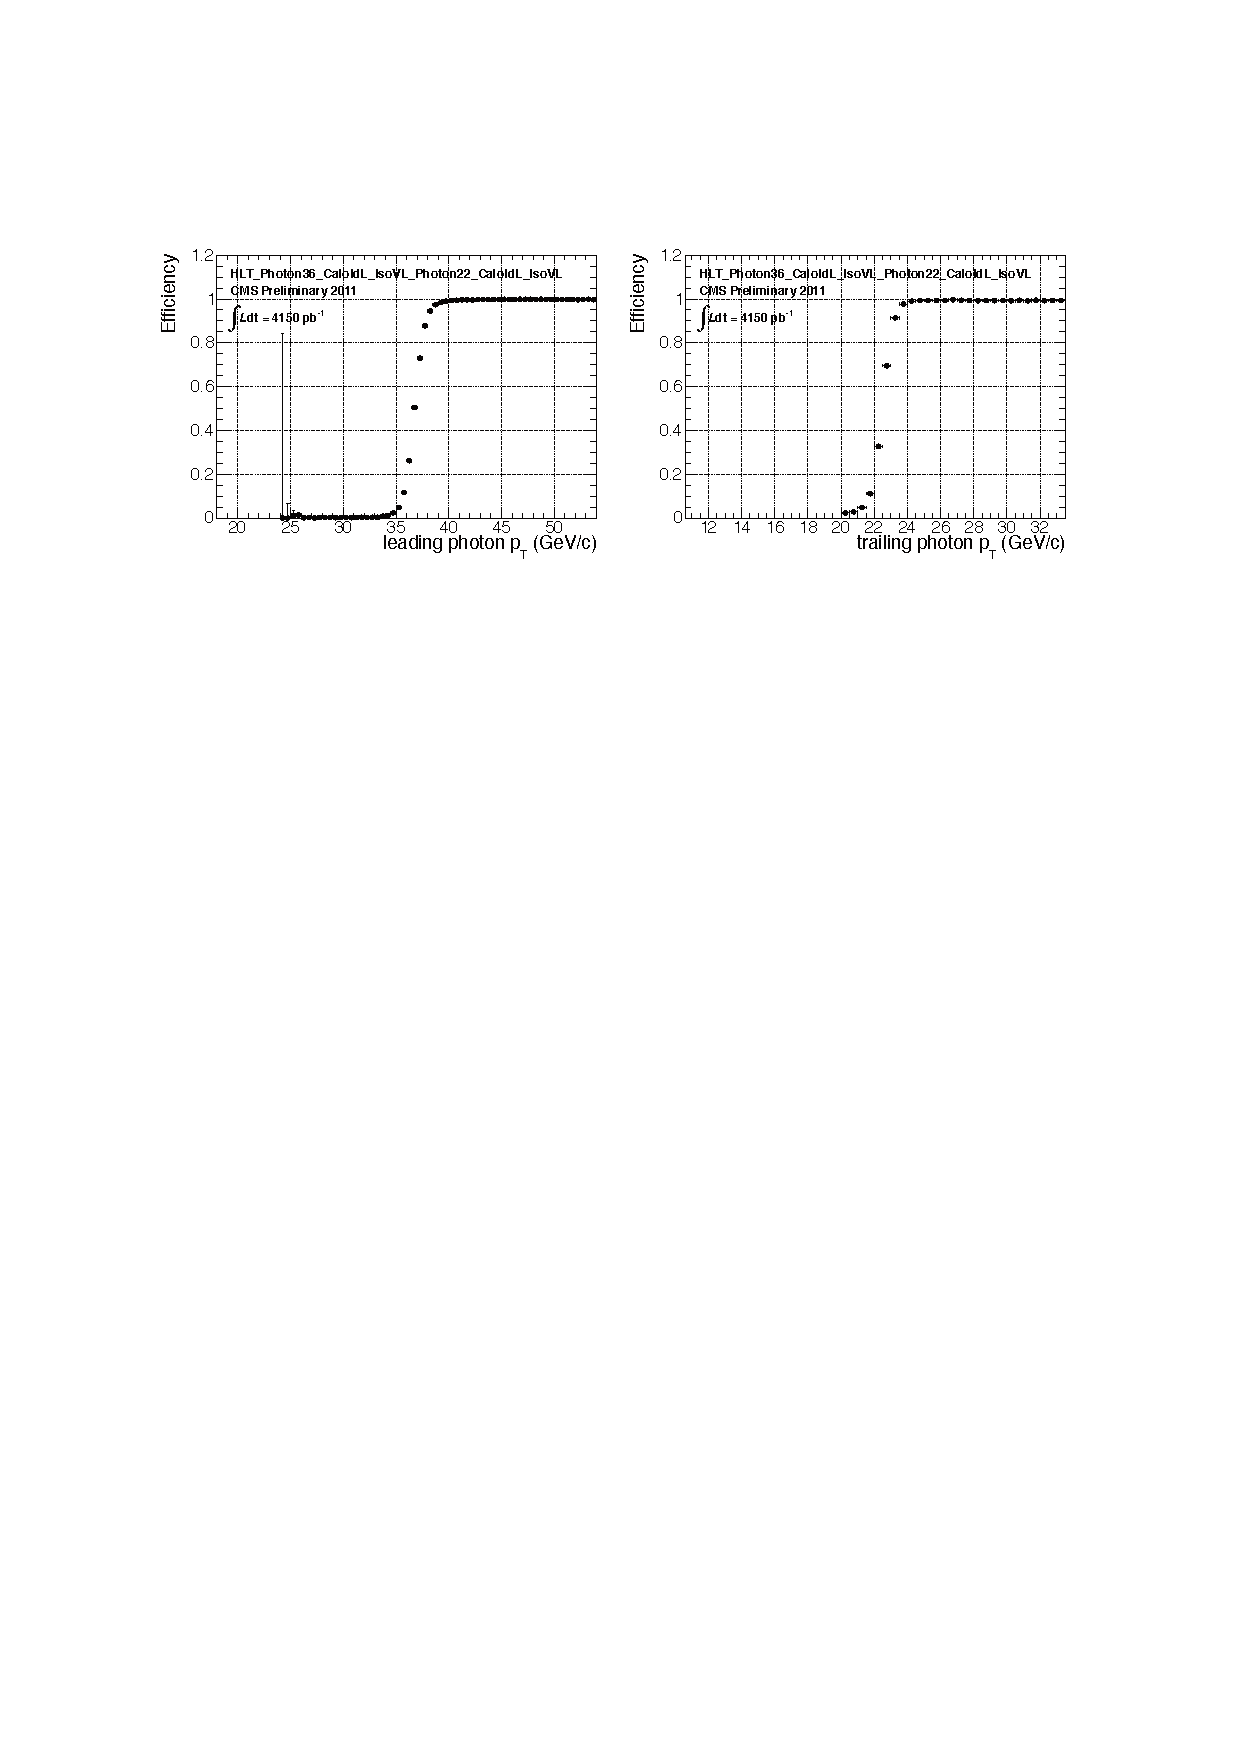
\includegraphics[scale=0.95]{HLT_efficiency}
	\caption{Efficiency of \texttt{HLT\_Photon36\_CaloIdL\_IsoVL\_Photon22\_CaloIdL\_IsoVL} for offline selected leading photon (left) and trailing photon (right) vs. photon $p_{T}$.  Reprinted from Fig. 2 of ref. \cite{CMS_AN-2011-515}.}
	\label{fig:HLT_efficiency}
\end{figure}

\section{Event Quality}
\label{sec:Event Quality}

To suppress instrumental backgrounds, a set of event quality cuts are applied to the $\gamma\gamma$, $e\gamma$, $ee$, and $\mathit{ff}$ samples.  First, all events are required to pass a good run selection, as determined by the CMS Physics Validation Team \cite{CMS_PVT}.  The good run selection excludes luminosity sections during which a sufficient part of the CMS detector was unpowered or malfunctioning.  Such conditions could occur if, for example, a high voltage supply trips off in the middle of a run, or a DAQ error corrupts data quality but is not spotted until after the data have been collected.  The severity of a detector problem is judged by its effect on a wide range of analyses and reconstruction algorithms.  Of the $\sim$ 5 $\mbox{fb}^{-1}$ of integrated luminosity delivered by the LHC in 2011, 4.68 $\mbox{fb}^{-1}$ passed the good run selection.  This analysis is performed on the entire 2011 certified dataset.

Second, all events must contain at least one good interaction vertex.  The criteria for a good vertex are:

\begin{itemize}
\item $\chi^{2} \neq 0\mbox{ OR}\mbox{ ndof} \neq 0\mbox{ OR}\mbox{ }N_{\mathrm{tracks}} \neq 0$, where $\chi^{2}$ and ndof are calculated for the track fit to the vertex, and $N_{\mathrm{tracks}}$ is the number of tracks in the vertex fit
\item $\mbox{ndof} > 4$
\item $|z| < 24$ cm, where $z$ is the $z$-coordinate of the vertex position
\item $|\rho| < 2$ cm, where $\rho$ is the transverse displacement of the vertex position from the beam line
\end{itemize}
%
The good vertex requirement eliminates non-collision backgrounds such as beam scraping, beam halo, cosmic muon interactions, and instrumental effects.

Third, the two electromagnetic objects in the $\gamma\gamma$, $e\gamma$, $ee$, and $\mathit{ff}$ events must be separated in $\phi$ by at least 0.05.  This requirement protects against beam halo bremsstrahlung, in which a halo muon traveling parallel to the beam line radiates an energetic photon while itself depositing a large amount of energy in the ECAL.  In this case, the two ECAL hits would likely be at the same $\phi$ (and $\rho$).

Fourth, the two EM objects must be separated in $R$ by at least 0.6.  Since the isolation cone size used is 0.3, this ensures that the isolation energy of one EM object cannot be in the veto strip (Fig.~\ref{fig:isolation_cones}) of the other.

Finally, the $\gamma\gamma$, $e\gamma$, $ee$, and $\mathit{ff}$ events must pass an HCAL noise filter and ECAL dead channel filter.  The HCAL noise filter guarantees that all HCAL reconstructed hits are inconsistent with any noise source.  Noise sources \cite{HCAL_noise_CRAFT} include:

\begin{itemize}
\item Ion feedback in the HPDs absent any true incident photons, in which a thermal electron ionizes a molecule in the HPD acceleration gap, faking a real signal
\item HPD discharge affecting nearly all channels in the same HPD \cite{HCAL_noise_AN}, partially explained by the effect of the 4 T CMS magnetic field on the flashover voltage of the dielectric \cite{Korzekwa}
\item Concurrent signals in nearly all 72 channels of a single RBX, as yet unexplained
\item HF PMT window hits (as opposed to the usual quartz fiber hits)
\item ADC saturation
\end{itemize}
%
Since HCAL noise may induce fake jets or \MET, events are rejected if any of the following criteria are true:

\begin{itemize}
\item Any HPD has $> 17$ hits
\item A single HPD has $> 10$ hits, but every other HPD has zero hits
\item An RBX has $> 10$ zero-ADC-count hits
\item Any HB/HE reconstructed hit corresponding to an RBX with $> 50$ GeV of energy fails a two-dimensional cut defined by the variables $(TS4 - TS5)/(TS4 + TS5)$ vs. $TS4 + TS5$, where $TS4$($TS5$) is the hit amplitude in the fourth(fifth) time sample read out for that hit.  The cut is defined in Fig.~\ref{fig:R45}.
\end{itemize}

\begin{figure}
	\centering
	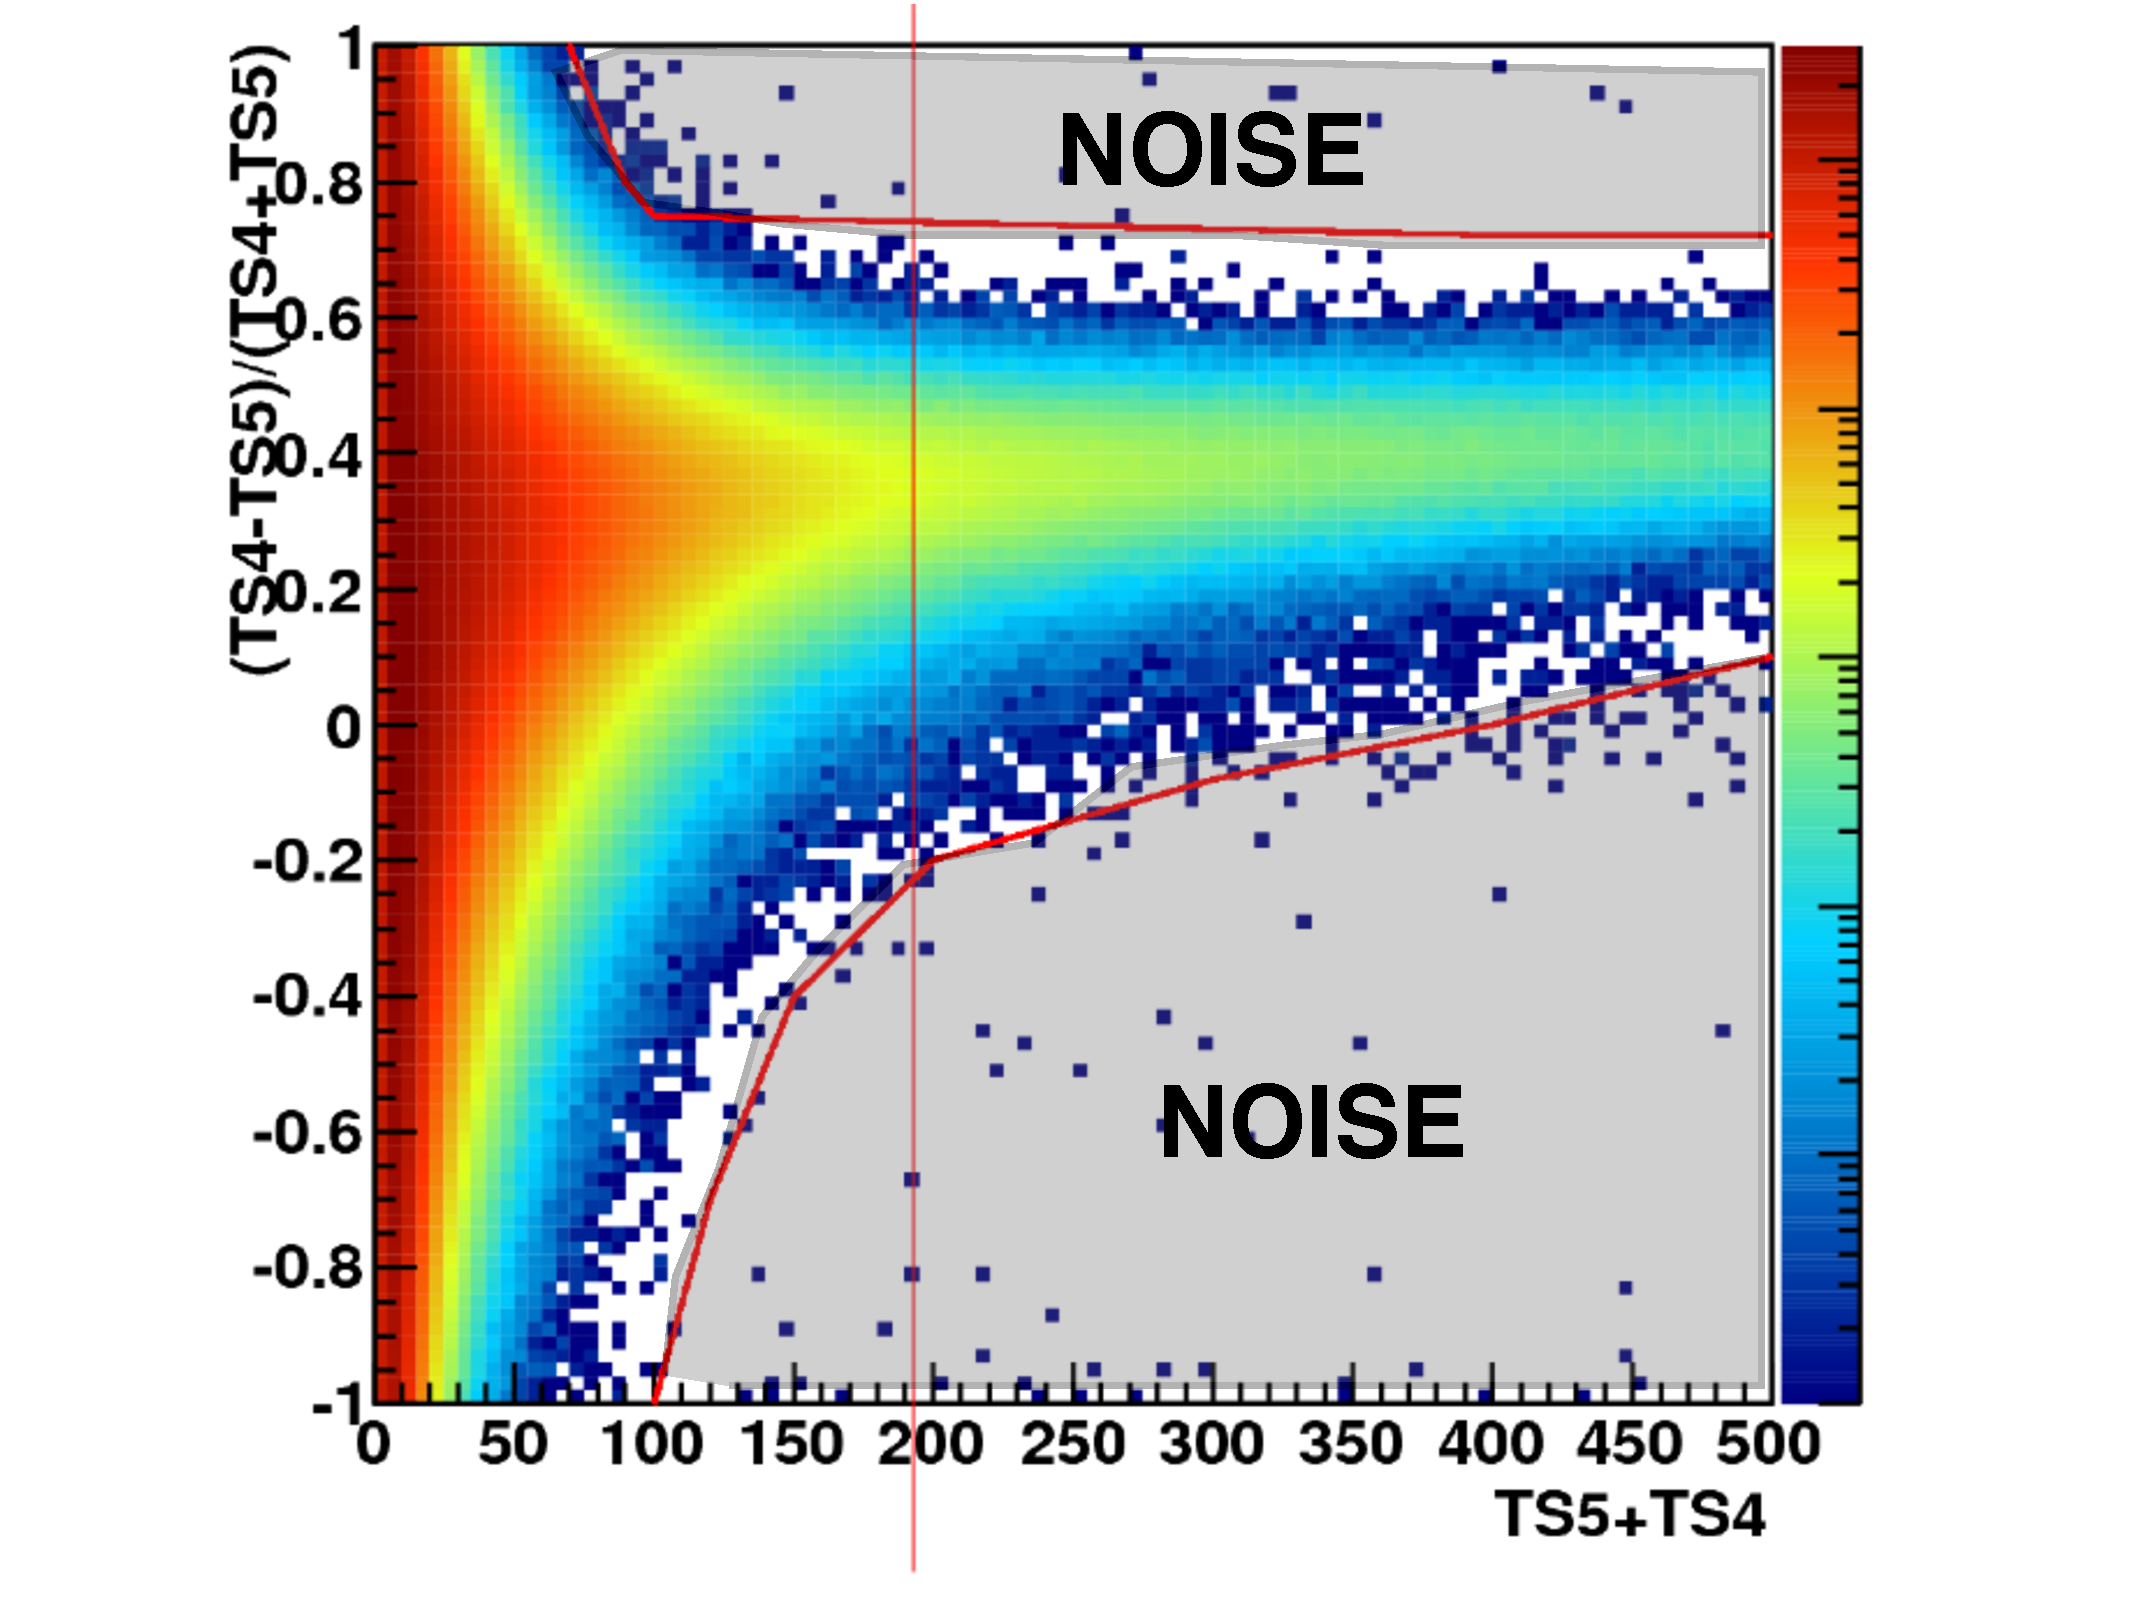
\includegraphics[scale=0.25]{R45}
	\caption{$(TS4 - TS5)/(TS4 + TS5)$ vs. $TS4 + TS5$ for a minimum bias sample.  HB/HE hits are considered noisy if they lie in the sparsely populated gray region labeled "NOISE" defined by the curved red lines.  Adapted from ref. \cite{Chen}.}
	\label{fig:R45}
\end{figure}

The ECAL dead channel filter is designed to flag events in which significant EM energy was deposited in a masked region of the ECAL by using the trigger primitive information for the corresponding trigger tower.  Energy deposited in a masked region of ECAL can cause fake \MET.  Events are rejected if the trigger primitive $E_{T}$ exceeds the maximum value of 63.75 GeV in any trigger tower that is masked in the readout.

\section{Photon Identification Efficiency}
\label{sec:Photon Identification Efficiency}

In order to determine the cross section (or cross section upper limit) for a GGM signal, the photon identification efficiency is needed.  Since no suitably large sample of $Z\rightarrow\mu\mu\gamma$ events in CMS exists yet, the efficiency calculation relies on the similarity between detector response to electrons and photons.  A scale factor to correct the MC photon ID efficiency to the real photon efficiency for the data is obtained from the ratio of the electron efficiency from the data to the electron efficiency from MC.  \marginpar{\textcolor{blue}{Removed reference to plots}}The different types of photon ID variables---calorimeter and track isolation, ratio of hadronic to electromagnetic energy of the shower, and transverse shower shape---are chosen so that their distributions for isolated electrons and photons are similar.\footnote{$R9$ differs between photons and radiating electrons, but the requirement $R9 < 1$ is loose enough not to introduce problems with the use of electrons to measure the photon ID efficiency.}

The photon selection efficiency is

\begin{eqnarray}
\label{eq:photon_ID_efficiency}
\epsilon_{\gamma} = \epsilon_{\gamma}^{\mathrm{MC}}\times\frac{\epsilon_{e}^{\mathrm{data}}}{\epsilon_{e}^{\mathrm{MC}}}
\end{eqnarray}
%
where

\begin{itemize}
  \item $\epsilon_{\gamma}$ is the photon ID efficiency in data,
  \item $\epsilon_{\gamma}^{\mathrm{MC}}$ is the photon ID efficiency in MC,
  \item $\epsilon_{e}^{\mathrm{data}}$ is the electron ID efficiency obtained using $Z\rightarrow ee$ electrons in the data that satisfy the photon ID cuts, and
  \item $\epsilon_{e}^{\mathrm{data}}$ is the electron ID efficiency obtained using $Z\rightarrow ee$ electrons in MC that satisfy the photon ID cuts.
\end{itemize}

The ratio $\epsilon_{e}^{\mathrm{data}}/\epsilon_{e}^{\mathrm{MC}}$ is defined as the scale factor by which the GGM signal MC photon ID efficiency must be multiplied to give an estimate of the photon ID efficiency in data.  The photon ID requirements of Table~\ref{tab:g_f_criteria} plus the \verb+IsoVL+ HLT requirement described in Sec.~\ref{sec:HLT} and Table~\ref{tab:HLT_by_run_range} are repeated in Table~\ref{tab:photon_ID_cuts}.

\begin{table}[hcbp]
\caption{Candidate photon ID requirements.}
\centering
\begin{tabular}{|c|c|}
\hline
Variable & Cut \\
\hline
\hline
$I_{\mathrm{ECAL}}$ & $< 0.012E_{T} + 6$ GeV \\
$I_{\mathrm{HCAL}}$ & $< 0.005E_{T} + 4$ GeV \\
$I_{\mathrm{track}}$ & $< 0.002E_{T} + 4$ GeV \\
\hline
$H/E$ & $< 0.05$ \\
\hline
$\sigma_{i\eta i\eta}$ & $< 0.011$ \\
\hline
\begin{tabular}[c]{@{}c@{}}$I_{\mathrm{ECAL}} - 0.0792\rho\mbox{ + }$\\$I_{\mathrm{HCAL}} - 0.0252\rho + I_{\mathrm{track}}$\end{tabular} & $< 6$ GeV \\
\hline
$R9$ & $< 1$ \\
\hline
\end{tabular}
\label{tab:photon_ID_cuts}
\end{table}

\subsection{Tag and Probe Method}
\label{sec:Tag_and_Probe_Method}

A \textit{tag and probe} method using $Z$ events is utilized to measure the efficiency of the photon ID cuts in Table~\ref{tab:g_f_criteria}.  The tag is a well-identified electron.  The probe, by contrast, is as loosely identified as possible, and all tags must pass the probe criteria in addition to the stringent tag criteria.  The tag and probe criteria used in this study are shown in Table~\ref{tab:tag_probe_cuts}.

\begin{table}[hcbp]
\caption{Tag and probe criteria.  The superscript 0.4 indicates that the isolation variable was calculated in a cone of $\Delta\mbox{R} = 0.4$ around the photon candidate.  The isolations without superscripts use the standard $\Delta\mbox{R} = 0.3$ cones.}
\centering
\begin{minipage}{\textwidth}
\centering
\begin{tabular}{|c|c|c|}
\hline
\multirow{2}{*}{Variable} & \multicolumn{2}{c|}{Cut} \\
\cline{2-3}
& Tag & Probe \\
\hline
\hline
RECO object & photon & photon \\
\hline
HLT & \begin{tabular}[c]{@{}c@{}}\texttt{HLT\_Ele17\_CaloIdVT\_CaloIsoVT\_TrkIdT\_}\\\texttt{TrkIsoVT\_SC8\_Mass30\_v*}\\(must have fired the 17 GeV leg)\end{tabular} & --- \\
\hline
$H/E$ & $< 0.05$ & $< 0.15$ \\
\hline
$I_{\mathrm{ECAL}}^{0.4}$ & $< 0.006E_{T} + 4.2$ GeV & --- \\
\hline
$I_{\mathrm{HCAL}}^{0.4}$ & $< 0.0025E_{T} + 2.2$ GeV & --- \\
\hline
$I_{\mathrm{track}}^{0.4}$ & $< 0.001E_{T} + 2.0$ GeV & --- \\
\hline
$E_{T}$ & $> 25$ GeV & --- \\
\hline
SC $E_{T}$ & --- & $> 15$ GeV \\
\hline
SC $|\eta|$ & $< 1.4442$ & $< 1.4442$ \\
\hline
$\sigma_{i\eta i\eta}$ & $< 0.009$ & --- \\
\hline
Has pixel seed & Yes & --- \\
\hline
Track match type & General track\footnote{A general track is reconstructed with the CMS standard combinatorial track finder \cite{CMS_NOTE_2006/041}.} & --- \\
\hline
Track match $\Delta$R & $< 0.04$ & --- \\
\hline
Track match $p_{T}$ & $> 15$ GeV & --- \\
\hline
Track match $|\eta|$ & $< 1.479$ & --- \\
\hline
\end{tabular}
\end{minipage}
\label{tab:tag_probe_cuts}
\end{table}

The invariant mass of the tag and probe are required to be within a narrow window around $Z$ mass.  Assuming that the probabilities of the tag and probe legs of the $Z$ decay to pass the photon ID cuts are uncorrelated, the efficiency can be estimated as

\begin{eqnarray}
\epsilon &=& \frac{N_{\mathrm{tag-pass}}}{N_{\mathrm{tag-pass}} + N_{\mathrm{tag-fail}}}
\end{eqnarray}
%
where $N_{\mathrm{tag-pass}}$ is the number of tag-probe pairs in which the probe leg passes the photon ID cuts under study and $N_{\mathrm{tag-fail}}$ is the number of tag-probe pairs in which the probe leg fails the cuts.  Implicit in these definitions is a double counting of pairs in which both electrons pass the tag and probe criteria \cite{tag_and_probe_method_AN}.  In addition, in the rare circumstance (less than 1\% in MC \cite{tag_and_probe_method_AN}) that two or more probes may be matched to one tag, the pair with invariant mass closest to the $Z$ mass is chosen.

In practice, $N_{\mathrm{tag-pass}}$ and $N_{\mathrm{tag-fail}}$ are returned by a simultaneous unbinned maximum likelihood fit to the invariant mass distributions of tag-pass and tag-fail events, with appropriate signal and background PDF assumptions.  The fit form used is

\begin{eqnarray}
f_{\mathrm{tag-pass}}(m_{\mathrm{tag-pass}}) &=& \epsilon N_{S}f_{S}^{\mathrm{pass}}(m_{\mathrm{tag-pass}}) + N_{B}^{\mathrm{pass}}f_{B}^{\mathrm{pass}}(m_{\mathrm{tag-pass}})\nonumber \\
f_{\mathrm{tag-fail}}(m_{\mathrm{tag-fail}}) &=& (1 - \epsilon) N_{S}f_{S}^{\mathrm{fail}}(m_{\mathrm{tag-fail}}) + N_{B}^{\mathrm{fail}}f_{B}^{\mathrm{fail}}(m_{\mathrm{tag-fail}})
\end{eqnarray}
%
where $f_{\mathrm{tag-pass}}(m_{\mathrm{tag-pass}})$ and $f_{\mathrm{tag-fail}}(m_{\mathrm{tag-fail}})$ are the tag-pass and tag-fail PDFs, respectively; $\epsilon$ is the efficiency; $N_{S}$ is the total number of $Z$ signal events summed over both samples; $f_{S}^{\mathrm{pass}}(m_{\mathrm{tag-pass}})$ and $f_{S}^{\mathrm{fail}}(m_{\mathrm{tag-fail}})$ are the tag-pass and tag-fail signal PDFs, respectively; $N_{B}^{\mathrm{pass}}$ and $N_{B}^{\mathrm{fail}}$ are the numbers of background events in the tag-pass and tag-fail samples, respectively; and $f_{B}^{\mathrm{pass}}(m_{\mathrm{tag-pass}})$ and $f_{B}^{\mathrm{fail}}(m_{\mathrm{tag-fail}})$ are the tag-pass and tag-fail background PDFs, respectively.  This particular implementation of the tag and probe methodology is based on tag \verb+CMSSW_4_2_5+ of the CMSSW package \verb+PhysicsTools/TagAndProbe+, and uses the MINUIT2 \cite{MINUIT} library, as coded in RooFit \cite{RooFit}, for the likelihood maximization.  For this study, CMSSWv4.2.8 was used.

For both samples, the signal shape is assumed to be a Crystal Ball function \cite{Crystal_Ball} convoluted with the $Z$ generated lineshape, while the background shape is a PDF that describes the falling background as well as the kinematic turn-on at low invariant mass.  The background PDF, called \verb+RooCMSShape+ \cite{tag_and_probe_method_AN}, is given by

\begin{eqnarray}
\label{eq:RooCMSShape}
f_{\mathrm{RooCMSShape}}(x) = \begin{cases} \mbox{1e20} & \mbox{for }(x - \mu)\gamma < -70 \\
\mbox{0} & \mbox{for }(x - \mu)\gamma > 70 \\
\mbox{erfc}((\alpha - x)\beta)\exp{(-(x - \mu)\gamma)} & \mbox{otherwise} \end{cases}
\end{eqnarray}
%
where $\alpha$, $\beta$, $\gamma$, and $\mu$ are parameters of the fit, most of which are held fixed.  In the three lowest $E_{T}$ bins, all parameters of the tag-pass and tag-fail background PDFs are left floating, because the effect of the relaxed $E_{T}$ cuts has a significant effect on the background shape.  More details of the signal and background PDFs are given in Table~\ref{tab:PDFs}.  The fixed signal and background parameter values were determined by fitting a small sample ($0.0 \leq \eta < 0.25$) of \verb+Fall11+ MC signal (\verb+DYJetsToLL+) and background (\verb+QCD_Pt-20to30_BCtoE+, \verb+QCD_Pt-30to80_BCtoE+, \verb+QCD_Pt-80to170_BCtoE+, \\\verb+GJet_Pt-20_doubleEMEnriched+, \verb+WJetsToLNu+, \verb+TTJets+) with parameters left floating.\footnote{See Appendix~\ref{chap:Monte Carlo Samples} for a discussion of the MC samples.}

\begin{table}[hcbp]
\caption{Parameter values (parameter definitions are in the text) for the signal and background PDFs for the different samples.  The background PDF applies to all efficiency bins except the four lowest $E_{T}$ bins, which use a floating \texttt{RooCMSShape} background.  When a bracketed range is given, the parameter is allowed to float within that range.  When a constant is given, the parameter is fixed to that constant.}
\centering
\begin{tabular}{|m{1.25cm}|m{1.25cm}|m{1.25cm}|m{1.25cm}|m{1.25cm}|m{1.25cm}|m{1.25cm}|m{1.25cm}|m{1.25cm}|}
\hline
& \multicolumn{4}{c|}{Crystal Ball fit parameters} & \multicolumn{4}{c|}{\texttt{RooCMSShape} fit parameters} \\
\hline
PDF & $\mu$ & $\sigma$ & $\alpha$ & n & $\mu$ & $\alpha$ & $\beta$ & $\gamma$ \\
\hline
Tag-pass signal & [-1.0, 1.0] & [1.0, 3.0] & 0.87 & 97.0 & N/A & N/A & N/A & N/A \\
\hline
Tag-fail signal & [-1.0, 1.0] & [1.0, 3.0] & 0.73 & 134.9 & N/A & N/A & N/A & N/A \\
\hline
Tag-pass background & N/A & N/A & N/A & N/A & 65.0 & 61.949 & 0.04750 & 0.01908 \\
\hline
Tag-fail background & N/A & N/A & N/A & N/A & $\alpha$ & [50.0, 100.0] & 0.065 & 0.048 \\
\hline
\end{tabular}
\label{tab:PDFs}
\end{table}

\marginpar{\textcolor{blue}{Added fits}}Some fit examples are shown in Figures~\ref{fig:low_ET_bin} and ~\ref{fig:mid-eta_bin}.  In Fig.~\ref{fig:low_ET_bin}, which shows fits to data and MC for 15 GeV $\leq$ probe $E_{T}$ $<$ 20 GeV, the kinematic turn-on is below the invariant mass range covered by the plot.  The exponentially falling background is easily seen underneath the signal, and is especially pronounced in the background-dominated tag-fail sample.

\begin{figure}
	\centering
	\subfloat[Data.]{\label{fig:low_ET_bin_data}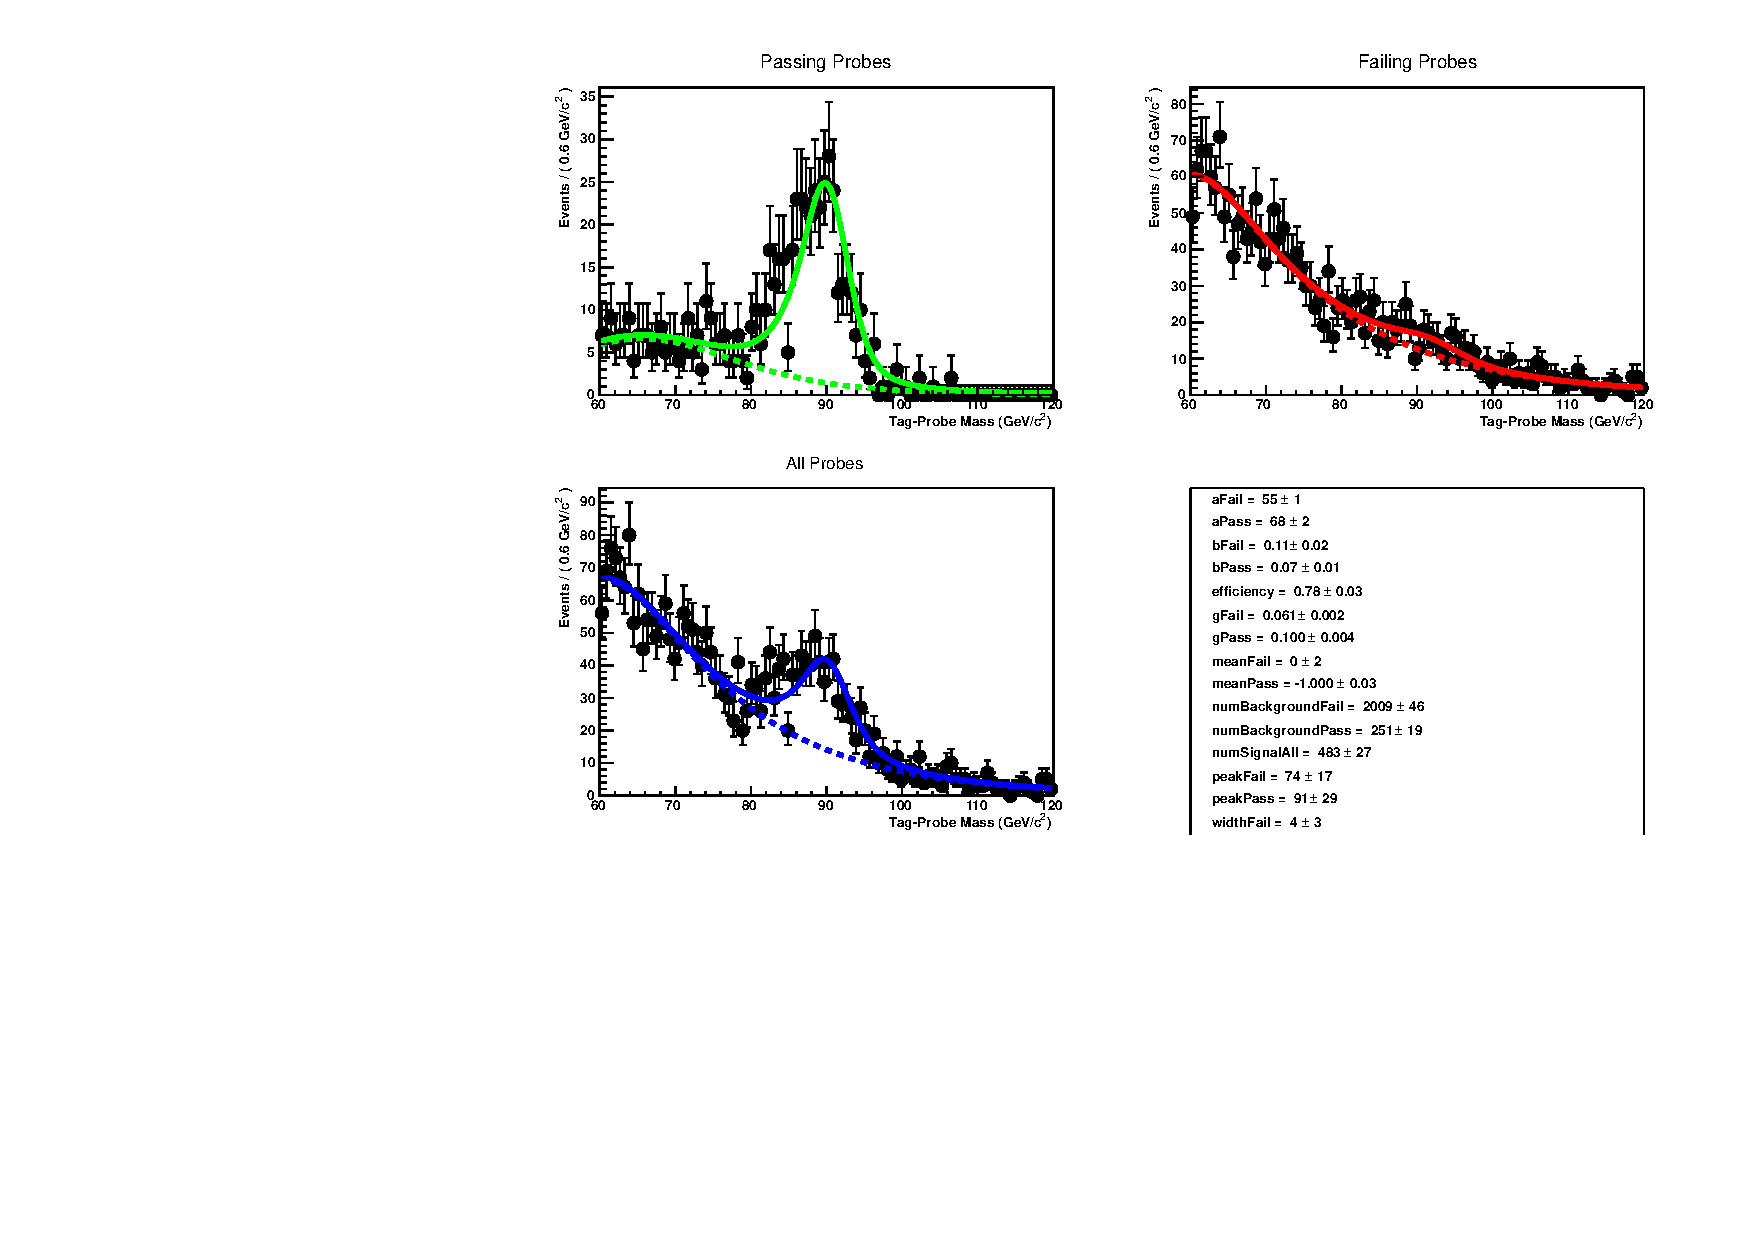
\includegraphics[scale=0.5]{low_ET_bin_data}}
	\\
	\subfloat[MC.  The purple points are the background MC (photon + jet, $W$, QCD, and $t\bar{t}$).]{\label{fig:low_ET_bin_MC}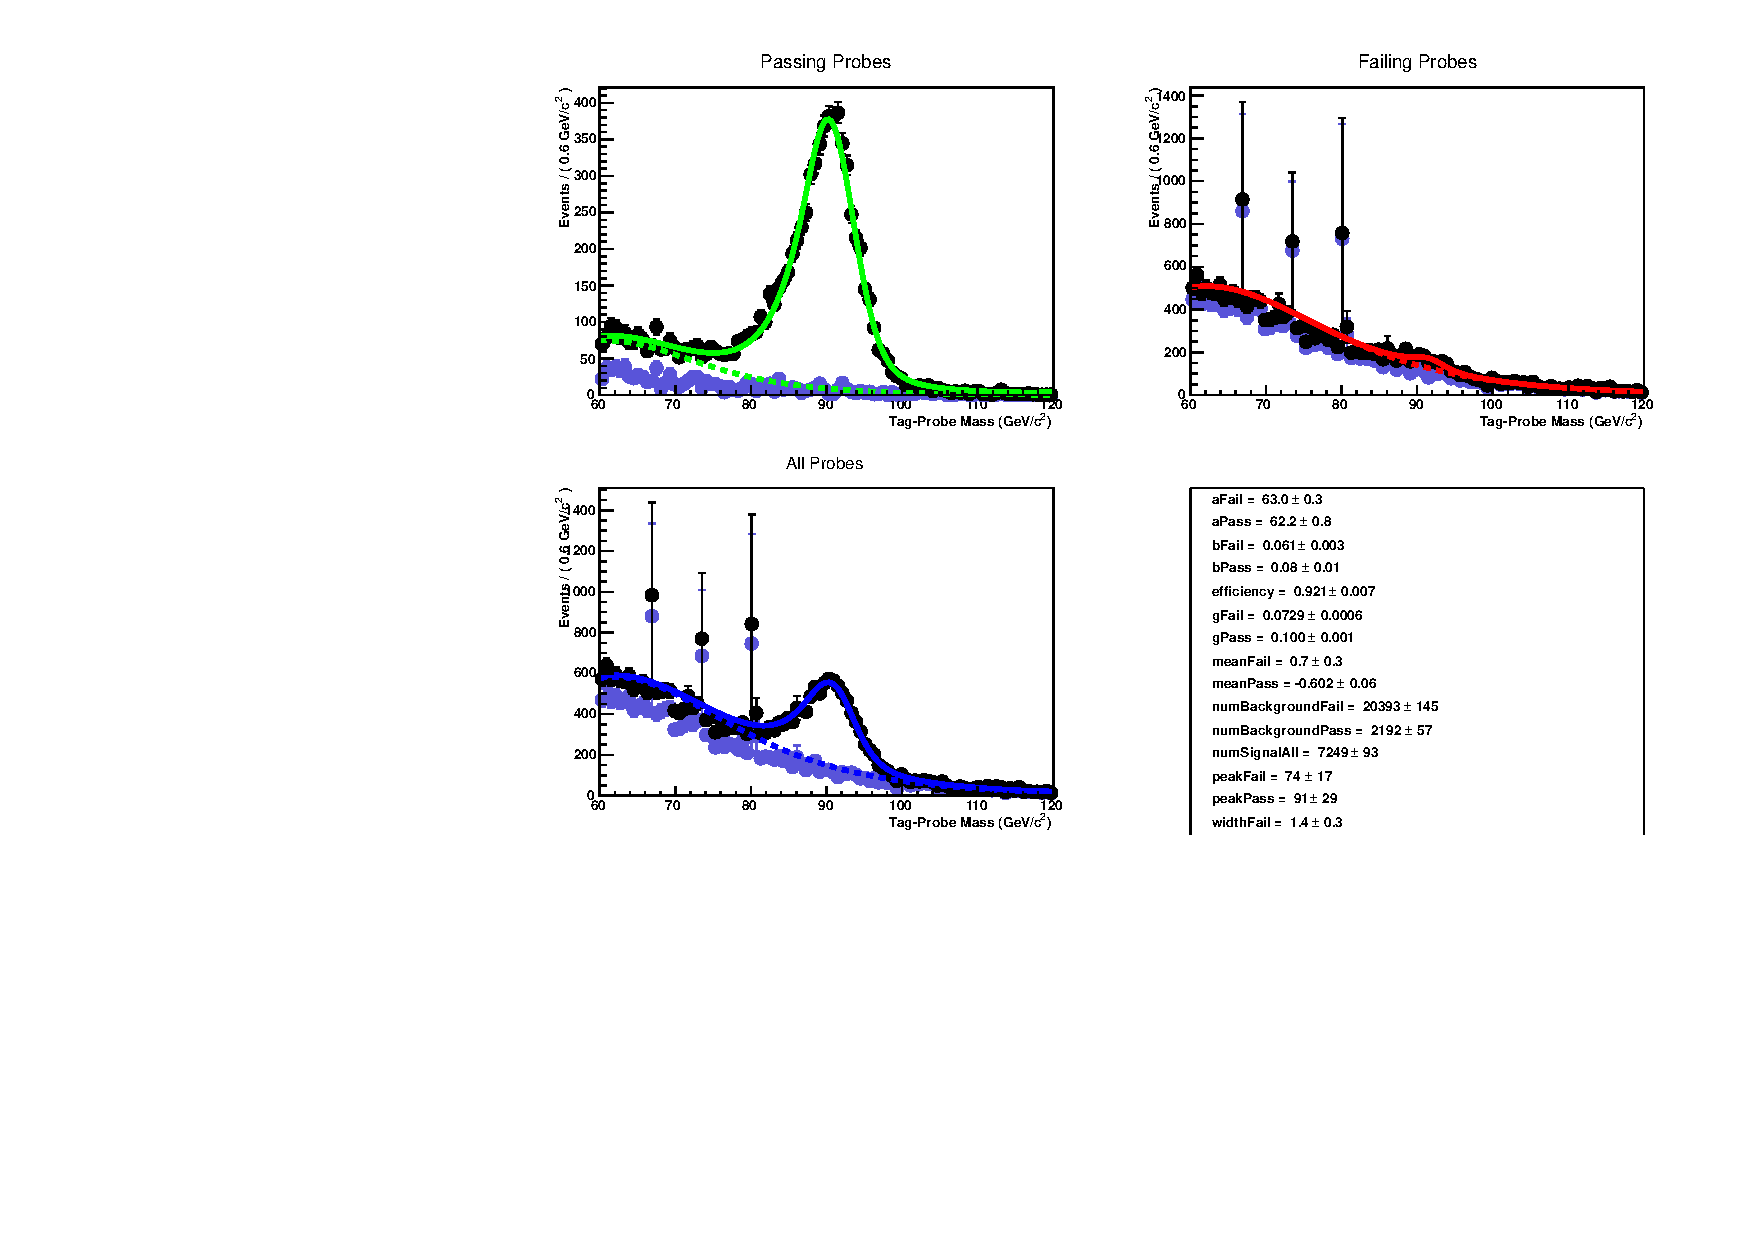
\includegraphics[scale=0.5]{low_ET_bin_MC}}
	\caption{Tag and probe invariant mass fits for 15 GeV $\leq$ probe $E_{T}$ $<$ 20 GeV.  Errors are statistical only.  The tag-pass fit is shown in green in the upper-left-hand plot, the tag-fail fit in red in the upper-right-hand plot, and a fit to both samples in blue in the lower-left-hand plot.  Dotted lines are the background components of the fits; solid lines are signal plus background.}
	\label{fig:low_ET_bin}
\end{figure}

\begin{figure}
	\centering
	\subfloat[Data.]{\label{fig:mid-eta_bin_data}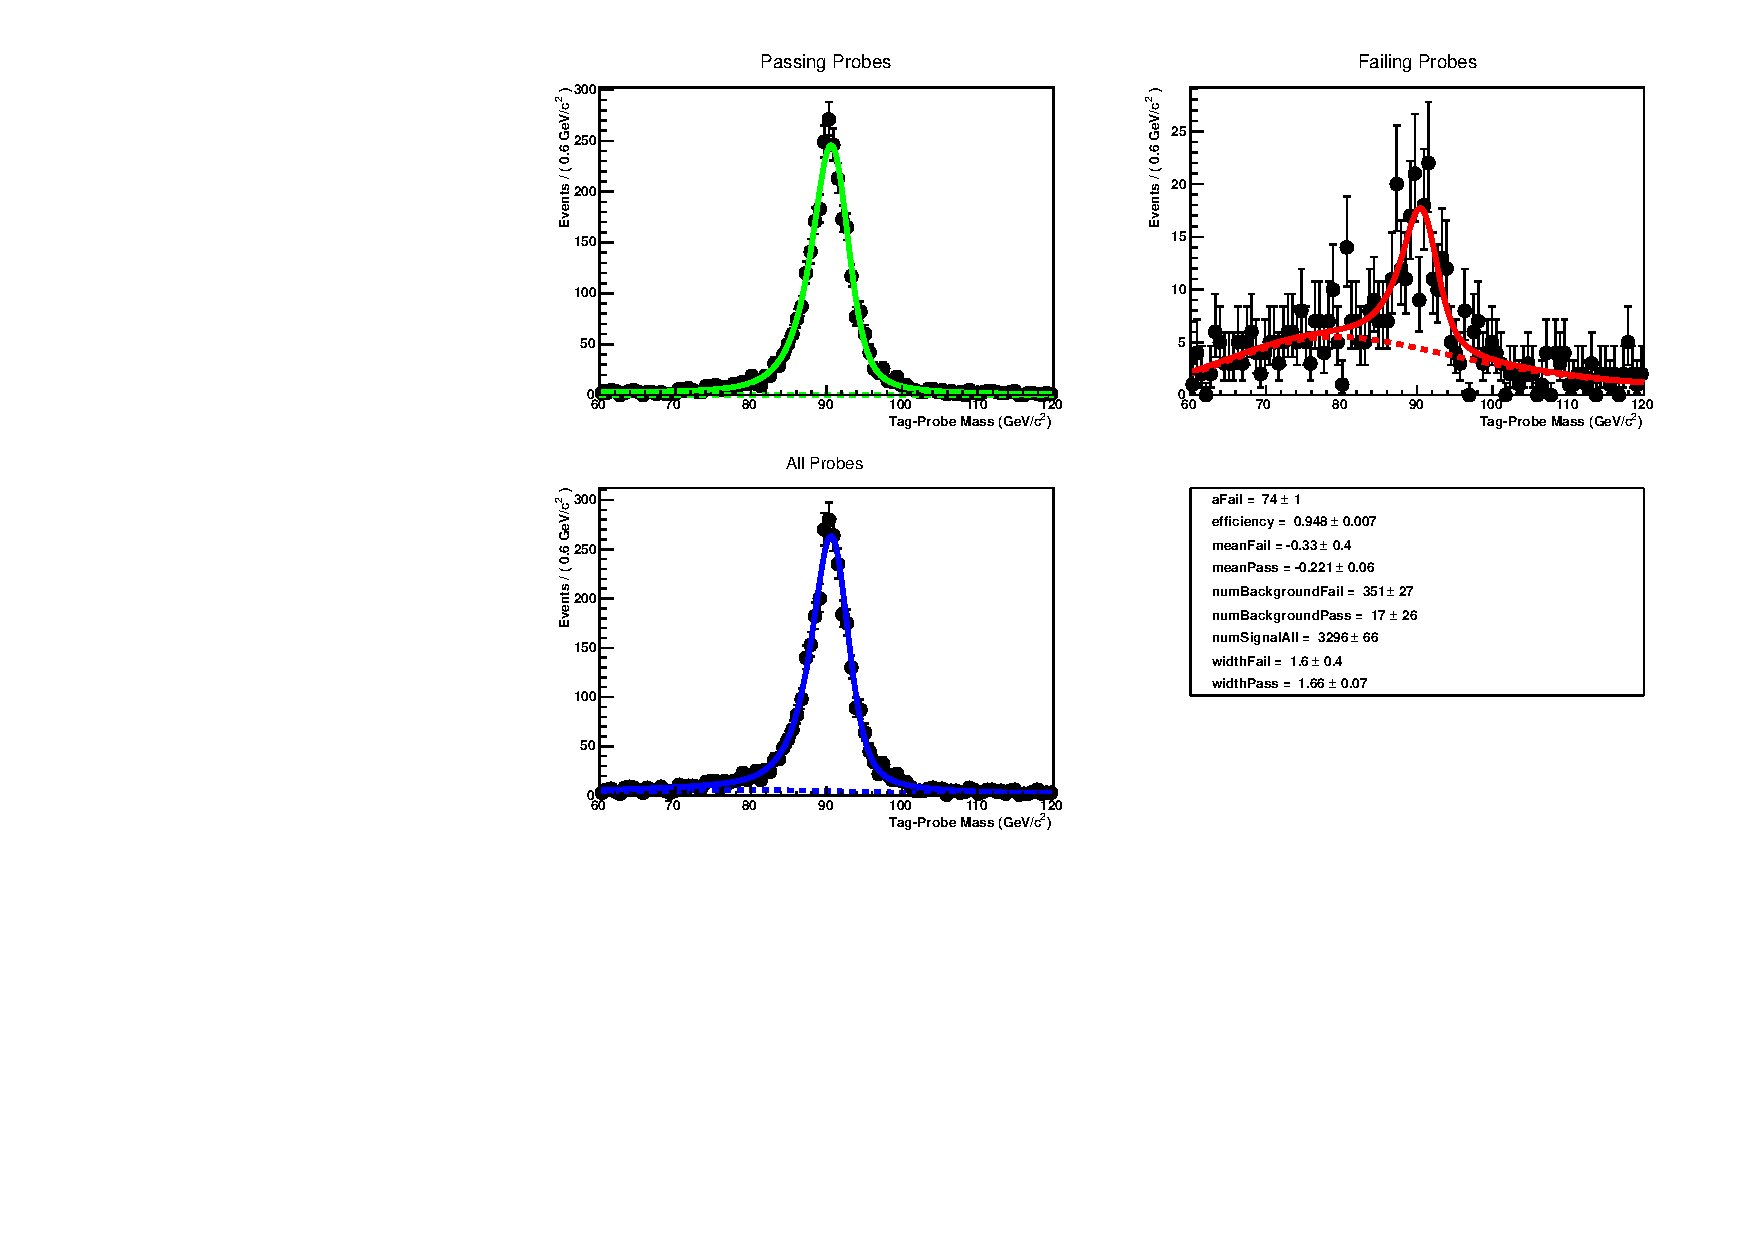
\includegraphics[scale=0.5]{mid-eta_bin_data}}
	\\
	\subfloat[MC.  The purple points are the background MC (photon + jet, $W$, QCD, and $t\bar{t}$).]{\label{fig:mid-eta_bin_MC}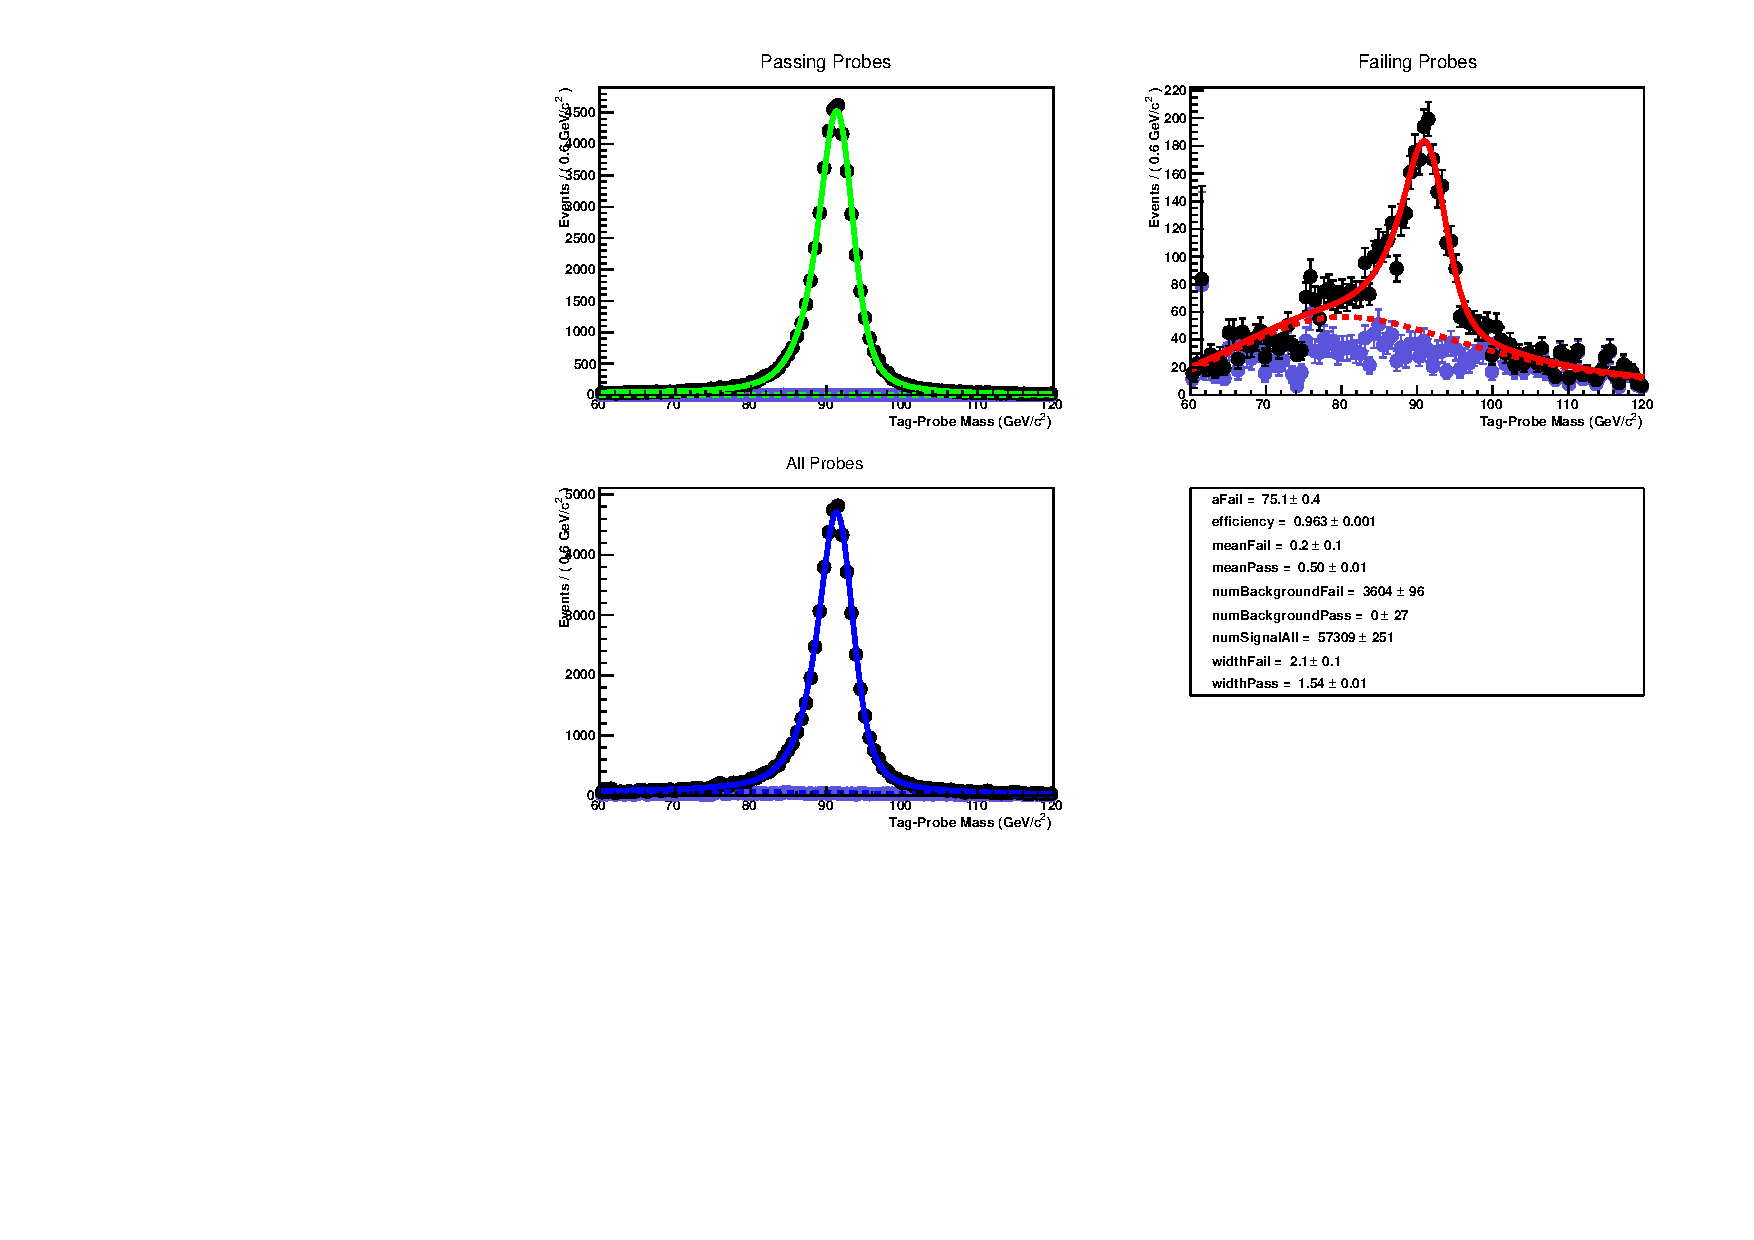
\includegraphics[scale=0.5]{mid-eta_bin_MC}}
	\caption{Tag and probe invariant mass fits for -0.25 $\leq$ probe $\eta$ $<$ -0.5.  Errors are statistical only.  The tag-pass fit is shown in green in the upper-left-hand plot, the tag-fail fit in red in the upper-right-hand plot, and a fit to both samples in blue in the lower-left-hand plot.  Dotted lines are the background components of the fits; solid lines are signal plus background.}
	\label{fig:mid-eta_bin}
\end{figure}

\subsection{Photon Efficiency Scale Factor $\epsilon_{e}^{\mathrm{data}}/\epsilon_{e}^{\mathrm{MC}}$}
\label{sec:Photon_Efficiency_Scale_Factor}

Figure~\ref{fig:scale_factors} shows the dependence of the photon ID efficiency scale factor $\epsilon_{e}^{\mathrm{data}}/\epsilon_{e}^{\mathrm{MC}}$ on $E_{T}$, $\eta$, and $N_{\mathrm{jet}}$, where jets are defined as in Table~\ref{tab:jet_definition_for_Nj_reweighting}, but with only the two $Z$ electrons considered as candidates for overlap removal.  Errors are statistical only.  There no significant dependence of the scale factor on these variables, so only one scale factor is computed from the entire dataset.

\begin{figure}
	\centering
	\subfloat[Scale factor vs. $E_{T}$.]{\label{fig:scale_factor_vs_ET}\includegraphics[scale=0.25]{scale_factor_vs_ET}}
	\hspace{1cm}
	\subfloat[Scale factor vs. $\eta$.]{\label{fig:scale_factor_vs_eta}\includegraphics[scale=0.25]{scale_factor_vs_eta}}
	\\
%	\subfloat[Scale factor vs. $\Delta R_{\gamma\mathrm{jet}}$.]{\label{fig:scale_factor_vs_dRPhotonJet}\includegraphics[scale=0.25]{scale_factor_vs_dRPhotonJet}}
%	\hspace{1cm}
	\subfloat[Scale factor vs. $N_{\mathrm{jet}}$.]{\label{fig:scale_factor_vs_Njet}\includegraphics[scale=0.25]{scale_factor_vs_Njet}}
	\caption{Dependence of the photon ID efficiency scale factor on some kinematic variables.  Errors are statistical only.}
	\label{fig:scale_factors}
\end{figure}

The effect of pileup is studied by comparing the efficiencies $\epsilon_{e}^{\mathrm{data}}$ and $\epsilon_{e}^{\mathrm{MC}}$ vs. the number of primary vertices ($N_{\mathrm{PV}}$) in the event.  The efficiency only drops a few percent for events with large $N_{\mathrm{PV}}$ after using pileup-corrected isolation cuts, as can be seen in Figure~\ref{fig:eff_vs_NPV}.  The MC tracks the data, and the scale factor is flat vs. $N_{\mathrm{PV}}$, as shown in Fig.~\ref{fig:scale_factor_vs_NPV}.

\begin{figure}
	\centering
	\subfloat[Data electron efficiency vs. $N_{\mathrm{PV}}$.]{\label{fig:eff_vs_NPV}\includegraphics[scale=0.25]{eff_vs_NPV}}
	\hspace{1cm}
	\subfloat[Scale factor vs. $N_{\mathrm{PV}}$.]{\label{fig:scale_factor_vs_NPV}\includegraphics[scale=0.25]{scale_factor_vs_NPV}}
	\caption{Dependence of the photon ID efficiency scale factor on the number of primary vertices per event.  Errors are statistical only.}
	\label{fig:vs_NPV}
\end{figure}

\marginpar{\textcolor{blue}{Official result uses this syst. error, so I am not rechecking it}}The scale factor is measured to be $\epsilon_{e}^{\mathrm{data}}/\epsilon_{e}^{\mathrm{MC}} = 0.994\mbox{ }\pm\mbox{ }0.002\mbox{(stat.) }\pm\mbox{ }0.035$(syst.).  Four main sources of systematic error, in addition to the statistical error of 0.2\%, were studied.

\begin{description}
  \item[Different behavior of electrons and photons in MC] Even though the photon ID cuts are designed to be similarly efficient for both electrons and photons, there might be a small difference in the performance between the two kinds of particles, e.g. because of electron bremsstrahlung.  To check this effect, the MC electron ID efficiency was calculated using a $Z\rightarrow ee$ sample and the MC photon ID efficiency was calculated using a $\gamma$ + jets sample.  Both samples were reconstructed in CMSSWv3.6.  Half the difference between these two results, 0.5\%, was taken as an error on the scale factor.
  \item[Pileup] \marginpar{\textcolor{blue}{Corrected some of these bullets}}To account for the possibility that the MC simulation may not adequately reproduce the data in a high pileup environment, the data/MC scale factor for events with 1-4 good reconstructed primary vertices was calculated, along with the same for events with $\geq$ 5 good reconstructed primary vertices.  The difference between the scale factors from both samples, 2.4\%, was taken as an error on the scale factor from pileup.
  \item[Signal fit over/underestimation] It was found that the signal fit slightly underestimates the data in the tag-pass sample, and slightly overestimates it in the tag-fail sample.  To cover this effect with a systematic error, the efficiencies in data and MC, and then the scale factor, were recalculated using the background (from fit) subtracted integrals of the tag-pass and tag-fail distributions, rather than the fitted signal yields in those distributions.  The difference between the scale factor found in this way and the nominal scale factor, 1.9\%, was taken as an error on the scale factor.
  \item[Signal and background shape assumption] To assess the magnitude of the error from the signal and background shape assumptions, the tag-pass and tag-fail tail parameters (Crystal Ball $\alpha$ and n) were varied by $\pm1\sigma$, and the background shape was varied between \verb+RooCMSShape+, exponential, power law, and quadratic.  All possible combinations of varied parameters were generated, and the data and MC were refit and new scale factors generated according to those combinations.  The error was taken as the largest deviation of the scale factor from nominal, 1.8\%.
\end{description}

Finally, the pixel veto efficiency was estimated from MC to be 0.96 $\pm$ 0.005(syst.), with error due to varying assumptions of the tracker material distribution \cite{CMS_AN-2010/271}.  In general, the photon ID selection used in this analysis is very efficient for GGM photons and robust to pileup, and its efficiency is fairly well measured.

\end{document}